% XeLaTeX

\documentclass{article}
\usepackage{ctex}
\usepackage{xypic}
\usepackage{amsfonts,amssymb}
\usepackage{multirow}
\usepackage{geometry}
\usepackage{graphicx}
\usepackage{listings}
\usepackage{lipsum}
\usepackage{courier}
\usepackage{fancyvrb}
\usepackage{etoolbox}


\linespread{1.2}
\geometry{left=3cm,right=2.5cm,top=2.5cm,bottom=2.5cm}

\makeatletter
\patchcmd{\FV@SetupFont}
  {\FV@BaseLineStretch}
  {\fontencoding{T1}\FV@BaseLineStretch}
  {}{}
\makeatother

\lstset{basicstyle=\small\fontencoding{T1}\ttfamily,breaklines=true}
\lstset{numbers=left,frame=shadowbox,tabsize=4}
%\lstset{extendedchars=false}
\begin{document}

\title{ICPC Templates For Africamonkey}
\author {Africamonkey}
\maketitle
\tableofcontents
\newpage
\section{莫队算法}
\subsection{普通莫队}
\begin{lstlisting}[language=C++]
struct Q { int l, r, sqrtl, id; } q[N];
int n, m, v[N], ans[N], nowans;
bool cmp(const Q &a, const Q &b) {
	if (a.sqrtl != b.sqrtl) return a.sqrtl < b.sqrtl;
	return a.r < b.r;
}
void change(int x) { if (!v[x]) checkin(); else checkout(); }
int main() {
	......
	for (int i=1;i<=m;i++) q[i].sqrtl = q[i].l / sqrt(n), q[i].id = i;
	sort(q+1, q+m+1, cmp);
	int L=1,R=0; nowans=0;
	memset(v, 0, sizeof(v));
	for (int i=1;i<=m;i++) {
		while (L<q[i].l) change(L++);
		while (L>q[i].l) change(--L);
		while (R<q[i].r) change(++R);
		while (R>q[i].r) change(R--);
		ans[q[i].id] = nowans;
	}
	......
}
\end{lstlisting}
\subsection{树上莫队}

\begin{lstlisting}[language=C++]
struct Query { int l, r, id, l_group; } query[N];
struct EDGE { int adj, next; } edge[N*2];
int n, m, top, gh[N], c[N], reorder[N], deep[N], father[N], size[N], son[N], Top[N];
void addedge(int x, int y) {
	edge[++top].adj = y;
	edge[top].next = gh[x];
	gh[x] = top;
}
void dfs(int x, int root=0) {
	reorder[x] = ++top; father[x] = root; deep[x] = deep[root] + 1;
	son[x] = 0; size[x] = 1; int dd = 0;
	for (int p=gh[x]; p; p=edge[p].next)
		if (edge[p].adj != root) {
			dfs(edge[p].adj, x);
			if (size[edge[p].adj] > dd) {
				son[x] = edge[p].adj;
				dd = size[edge[p].adj];
			}
			size[x] += size[edge[p].adj];
		}
}
void split(int x, int tp) {
	Top[x] = tp;
	if (son[x]) split(son[x], tp);
	for (int p=gh[x]; p; p=edge[p].next)
		if (edge[p].adj != father[x] && edge[p].adj != son[x])
			split(edge[p].adj, edge[p].adj);
}
int lca(int x, int y) {
	int tx = Top[x], ty = Top[y];
	while (tx != ty) {
		if (deep[tx] < deep[ty]) {
			swap(tx, ty);
			swap(x, y);
		}
		x = father[tx];
		tx = Top[x];
	}
	if (deep[x] < deep[y]) swap(x, y);
	return y;
}
bool cmp(const Query &a, const Query &b) {
	if (a.l_group != b.l_group) return a.l_group < b.l_group;
	return reorder[a.r] < reorder[b.r];
}
int v[N], ans[N];
void upd(int x) { if (!v[x]) checkin(); else checkout(); }
void go(int &u, int taru, int v) {
	int lca0 = lca(u, taru);
	int lca1 = lca(u, v);	upd(lca1);
	int lca2 = lca(taru, v); upd(lca2);
	for (int x=u; x!=lca0; x=father[x]) upd(x);
	for (int x=taru; x!=lca0; x=father[x]) upd(x);
	u = taru;
}
int main() {
	memset(gh, 0, sizeof(gh));
	scanf("%d%d", &n, &m); top = 0;
	for (int i=1;i<n;i++) {
		int x,y; scanf("%d%d", &x, &y);
		addedge(x, y); addedge(y, x);
	}
	top = 0; dfs(1); split(1, 1);
	for (int i=1;i<=m;i++) {
		if (reorder[query[i].l] > reorder[query[i].r]) 
			swap(query[i].l, query[i].r);
		query[i].id = i;
		query[i].l_group = reorder[query[i].l] / sqrt(n);
	}
	sort(query+1, query+m+1, cmp);
	int L=1,R=1; upd(1);
	for (int i=1;i<=m;i++) {
		go(L,query[i].l,R);
		go(R,query[i].r,L);
		ans[query[i].id] = answer();
	}
	......
}
\end{lstlisting}

\section{字符串}
\subsection{哈希}
\begin{lstlisting}[language=C++]
const int P=31,D=1000173169;
int n, pow[N], f[N]; char a[N];
int hash(int l, int r) { return (LL)(f[r]-(LL)f[l-1]*pow[r-l+1]%D+D)%D; }
int main() {
	scanf("%d%s", &n, a+1);
	pow[0] = 1;
	for (int i=1;i<=n;i++) pow[i] = (LL)pow[i-1]*P%D;
	for (int i=1;i<=n;i++) f[i] = (LL)((LL)f[i-1]*P+a[i])%D;
}
\end{lstlisting}
\subsection{KMP}
接口: void kmp(int n, char *a, int m, char *b); 

输入: 模式串长度 $n$ ,模式串 $a$ ,匹配串长度 $m$ ,匹配串 $b$

输出: 依次输出每个匹配成功的\emph{起始}位置

下标从 $0$ 开始。

\begin{lstlisting}[language=C++]
void kmp(int n, char* a, int m, char *b) {
    int i, j;
    for (nxt[0] = j = -1, i = 1; i < n; nxt[i++] = j) {
        while (~j && a[j + 1] != a[i]) j = nxt[j];
        if (a[j + 1] == a[i]) ++j;
    }
    for (j = -1, i = 0; i < m; ++i) {
        while (~j && a[j + 1] != b[i]) j = nxt[j];
        if (a[j + 1] == b[i]) ++j;
        if (j == n - 1) {
            printf("%d\n", i - (n - 1) + 1);
            j = nxt[j];
        }
    }
}
\end{lstlisting}
\subsection{可动态修改的KMP}
支持:加入一个字符,删除一个字符。

时间复杂度: $O(n \alpha)$ , $\alpha$ 为字符集大小。

代码中的字符为 $'0' - '9'$ ,可自行修改为 $'a' - 'z'$
\begin{lstlisting}[language=C++]
char t[N];
int top, nxt[N], nxt_l[N][10];
inline void del_letter() { --top; }
inline void add_letter(char x) {
	t[top++] = x;
	int j = top-1;
	memset(nxt_l[top], 0, sizeof(nxt_l[top]));
	nxt[top] = nxt_l[top-1][x-'0'];
	memcpy(nxt_l[top], nxt_l[nxt[top]], sizeof(nxt_l[nxt[top]]));
	nxt_l[top][t[nxt[top]]-'0'] = nxt[top]+1;
}
\end{lstlisting}
\subsection{扩展KMP}
接口: void ExtendedKMP(char *a, char *b, int *next, int *ret); 

输出: 

next:  a 关于自己每个后缀的最长公共前缀 

ret: a 关于 b 的每个后缀的最长公共前缀


EXKMP的next[i]表示:从i到n-1的字符串st前缀和原串前缀的最长重叠长度。

\begin{lstlisting}[language=C++]
void get_next(char *a, int *next) {
	int i, j, k;
	int n = strlen(a);
	for (j = 0; j+1<n && a[j]==a[j+1];j++);
	next[1] = j;
	k = 1;
	for (i=2;i<n;i++) {
		int len = k+next[k], l = next[i-k];
		if (l < len-i) {
			next[i] = l;
		} else {
			for (j = max(0, len-i);i+j<n && a[j]==a[i+j];j++);
			next[i] = j;
			k = i;
		}
	}
}
void ExtendedKMP(char *a, char *b, int *next, int *ret) {
	get_next(a, next);
	int n = strlen(a), m = strlen(b);
	int i, j, k;
	for (j=0;j<n && j<m && a[j]==b[j];j++);
	ret[0] = j;
	k = 0;
	for (i=1;i<m;i++) {
		int len = k+ret[k], l = next[i-k];
		if (l < len-i) {
			ret[i] = l;
		} else {
			for (j = max(0, len-i);j<n && i+j<m && a[j]==b[i+j];j++);
			ret[i] = j;
			k = i;
		}
	}
}
\end{lstlisting}

\subsection{Manacher}
p[i] 表示以 i 为对称轴的最长回文串长度
\begin{lstlisting}[language=C++]
char st[N*2], s[N];
int len, p[N*2];

while (scanf("%s", s) != EOF) {
	len = strlen(s);
	st[0] = '$', st[1] = '#';
	for (int i=1;i<=len;i++)
		st[i*2] = s[i-1], st[i*2+1] = '#';
	len = len * 2 + 2;
	int mx = 0, id = 0, ans = 0;
	for (int i=1;i<=len;i++) {
		p[i] = (mx > i) ? min(p[id*2-i]+1, mx-i) : 1;
		for (; st[i+p[i]] == st[i-p[i]]; ++p[i]) ;
		if (p[i]+i > mx) mx = p[i]+i, id = i;
		p[i] --;
		if (p[i] > ans) ans = p[i];
	}
	printf("%d\n", ans);
}
\end{lstlisting}
\subsection{最小表示法}
\begin{lstlisting}[language=C++]
string smallestRepresation(string s) {
	int i, j, k, l;
	int n = s.length();
	s += s;
	for (i=0,j=1;j<n;) {
		for (k=0;k<n && s[i+k]==s[j+k];k++);
		if (k>=n) break;
		if (s[i+k]<s[j+k]) j+=k+1;
		else {
			l=i+k;
			i=j;
			j=max(l,j)+1;
		}
	}
	return s.substr(i, n);
}
\end{lstlisting}

\subsection{AC自动机}
\begin{lstlisting}[language=C++]
struct Node {
	int next[**Size of Alphabet**];
	int terminal, fail;
} node[**Number of Nodes**];
int top;
void add(char *st) {
	int len = strlen(st), x = 1;
	for (int i=0;i<len;i++) {
		int ind = trans(st[i]);
		if (!node[x].next[ind])
			node[x].next[ind] = ++top;
		x = node[x].next[ind];
	}
	node[x].terminal = 1;
}
int q[**Number of Nodes**], head, tail;
void build() {
	head = 0, tail = 1; q[1] = 1;
	while (head != tail) {
		int x = q[++head];
		/*(when necessary) node[x].terminal |= node[node[x].fail].terminal; */
		for (int i=0;i<n;i++)
			if (node[x].next[i]) {
				if (x == 1) node[node[x].next[i]].fail = 1;
				else {
					int y = node[x].fail;
					while (y) {
						if (node[y].next[i]) {
							node[node[x].next[i]].fail = node[y].next[i];
							break;
						}
						y = node[y].fail;
					}
					if (!node[node[x].next[i]].fail) node[node[x].next[i]].fail = 1;
				}
				q[++tail] = node[x].next[i];
			}
	}
}
\end{lstlisting}

\subsection{后缀数组}
\subsubsection{倍增算法}
参数 m 表示字符集的大小,即 $0 \leq r_i < m$ 
\begin{lstlisting}[language=C++]
#define rank rank2
int n, r[N], wa[N], wb[N], ws[N], sa[N], rank[N], height[N];
int cmp(int *r, int a, int b, int l, int n) {
	if (r[a]==r[b]) {
		if (a+l<n && b+l<n && r[a+l]==r[b+l])
			return 1;
	}
	return 0;
}
void suffix_array(int m) {
	int i, j, p, *x=wa, *y=wb, *t;
	for (i=0;i<m;i++) ws[i]=0;
	for (i=0;i<n;i++) ws[x[i]=r[i]]++;
	for (i=1;i<m;i++) ws[i]+=ws[i-1];
	for (i=n-1;i>=0;i--) sa[--ws[x[i]]]=i;
	for (j=1,p=1;p<n;m=p,j<<=1) {
		for (p=0,i=n-j;i<n;i++) y[p++]=i;
		for (i=0;i<n;i++) if (sa[i]>=j) y[p++]=sa[i]-j;
		for (i=0;i<m;i++) ws[i]=0;
		for (i=0;i<n;i++) ws[x[y[i]]]++;
		for (i=1;i<m;i++) ws[i]+=ws[i-1];
		for (i=n-1;i>=0;i--) sa[--ws[x[y[i]]]]=y[i];
		for (t=x,x=y,y=t,x[sa[0]]=0,i=1,p=1;i<n;i++)
			x[sa[i]]=cmp(y,sa[i-1],sa[i],j,n)?p-1:p++;
	}
	for (i=0;i<n;i++) rank[sa[i]]=i;
	rank[n] = -1;
}
void calc_height() {
	int j=0;
	for (int i=0;i<n;i++)
		if (rank[i])
		{
			while (r[i+j]==r[sa[rank[i]-1]+j]) j++;
			height[rank[i]]=j;
			if (j) j--;
		}
}
\end{lstlisting}
\subsubsection{DC3算法}
注意:

$N$ 至少为字符串长度的 $3$ 倍

接口: suffix\_array(int *r, int *sa, int n, int m); 

r 表示字符串, sa 为后缀数组输出,$n$ 表示字符串长度,下标从 $0$ 开始。$m$ 为字符集大小。
\begin{lstlisting}[language=C++]
#define F(x) ((x)/3 + ((x)%3 == 1 ? 0:tb))
#define G(x) ((x) < tb ? (x)*3+1 : ((x)-tb)*3 + 2)
#define rank rank2

int r[N], wa[N], wb[N], ws[N], wv[N], sa[N], rank[N];

int c0(int *r,int a,int b) {
    return r[a]==r[b]&&r[a+1]==r[b+1]&&r[a+2]==r[b+2];
}

int c12(int k,int *r,int a,int b) {
    if(k==2) return r[a]<r[b]||r[a]==r[b]&&c12(1,r,a+1,b+1);
    else return r[a]<r[b]||r[a]==r[b]&&wv[a+1]<wv[b+1];
}

void dsort(int *r,int *a,int *b,int n,int m) {
    int i;for(i=0;i<n;i++) wv[i]=r[a[i]];
    for(i=0;i<m;i++) ws[i]=0;
    for(i=0;i<n;i++) ws[wv[i]]++;
    for(i=1;i<m;i++) ws[i]+=ws[i-1];
    for(i=n-1;i>=0;i--) b[--ws[wv[i]]]=a[i];
}

void dc3(int *r,int *sa,int n,int m) {
    int i,j,*rn=r+n,*san=sa+n,ta=0,tb=(n+1)/3,tbc=0,p;
    r[n]=r[n+1]=0;
    for(i=0;i<n;i++) if(i%3!=0) wa[tbc++]=i;
    dsort(r+2,wa,wb,tbc,m);
    dsort(r+1,wb,wa,tbc,m);
    dsort(r,wa,wb,tbc,m);
    for(p=1,rn[F(wb[0])]=0,i=1;i<tbc;i++) rn[F(wb[i])]=c0(r,wb[i-1],wb[i])?p-1:p++;
    if(p<tbc) dc3(rn,san,tbc,p);
    else for(i=0;i<tbc;i++) san[rn[i]]=i;
    for(i=0;i<tbc;i++) if(san[i]<tb) wb[ta++]=san[i]*3;
    if(n%3==1) wb[ta++]=n-1;
    dsort(r,wb,wa,ta,m);
    for(i=0;i<tbc;i++) wv[wb[i]=G(san[i])]=i;
    for(i=0,j=0,p=0;i<ta && j<tbc;p++)sa[p]=c12(wb[j]%3,r,wa[i],wb[j])?wa[i++]:wb[j++];
    for(;i<ta;p++) sa[p]=wa[i++];
    for(;j<tbc;p++) sa[p]=wb[j++];
}

void suffix_array(int *r, int *sa, int n, int m) {
    dc3(r, sa, n + 1, m);
    int top = 0;
    for (int i = 0; i < n + 1; ++i)
        if (sa[i] < n) sa[top++] = sa[i];
    for (int i = 0; i < n; ++i) rank[sa[i]] = i;
    rank[n] = -1;
}
\end{lstlisting}
\subsubsection{小技巧:拼接字符串}
接口: 

int gao1(int l, int r, int c, int p); 区间 $[l, r)$ 中保证第 $0$ 位到第 $c - 1$ 位都是相同的(设为字符串 $s$ ),现在我们在 $s$ 后面接一个字符 $p$ ,得到一个新的字符串 $s'$ 。返回值为最小的 $k$ 满足后缀 $sa[k]$ 前 $c + 1$ 位为 $s'$ 

int gao2(int l, int r, int c, int p); 区间 $[l, r)$ 中保证第 $0$ 位到第 $c - 1$ 位都是相同的(设为字符串 $s$ ),现在我们在 $s$ 后面接一个后缀 $sa[p]$ ,得到一个新的字符串 $s'$ 。返回值为最小的 $k$ 满足后缀 $sa[k]$ 前 $c + len(sa[p])$ 位为 $s'$ 

\begin{lstlisting}[language=C++]
int gao1(int l,int r,int c,int p) {
        --l;
        while (l+1<r) {
                int md=(l+r)>>1;
                if (sa[md]+c<n&&s[sa[md]+c]>=p) r=md; else l=md;
        }
        return r;
}
int gao2(int l,int r,int c,int p) {
        --l;
        while (l+1<r) {
                int md=(l+r)>>1;
                if (sa[md]+c<=n&&rk[sa[md]+c]>=p) r=md; else l=md;
        }
        return r;
}
\end{lstlisting}
示例调用:
\begin{lstlisting}[language=C++]
suf1[m] = -1, suf2[m] = n;
for (int i = m - 1; i >= 0; --i) {
	int l = gao1(0, n, 0, t[i]), r = gao1(0, n, 0, t[i]);
	suf1[i] = gao2(l, r, 1, suf1[i + 1]);
	suf2[i] = gao2(l, r, 1, suf2[i + 1]);
}
\end{lstlisting}
\subsection{后缀自动机}
下面的代码是求两个串的LCS(最长公共子串)。
\begin{lstlisting}[language=C++]
#include <bits/stdc++.h>

#define N 500001
#define M (N << 1)

using namespace std;

char st[N];
int pre[M], son[26][M], step[M], refer[M], size[M], tmp[M], topo[M], last, total;

int apply(int x, int now) {
	step[++total] = x;
	refer[total] = now;
	return total;
}

void extend(char x, int now) {
	int p = last, np = apply(step[last]+1, now);
	size[np] = 1;
	for (; p && !son[x][p]; p=pre[p]) son[x][p] = np;
	if (!p) pre[np] = 1;
	else {
		int q = son[x][p];
		if (step[p]+1 == step[q]) pre[np] = q;
		else {
			int nq = apply(step[p]+1, now);
			for (int i=0;i<26;i++) son[i][nq] = son[i][q];
			pre[nq] = pre[q];
			pre[q] = pre[np] = nq;
			for (; p && son[x][p]==q; p=pre[p]) son[x][p] = nq;
		}
	}
	last = np;
}
void init() {
	last = total = 0;
	last = apply(0, 0);
	scanf("%s",st);
	int n = strlen(st);
	for (int i = 0; i <= n * 2; ++i) {
		pre[i] = step[i] = refer[i] = size[i] = tmp[i] = topo[i] = 0;
		for (int j = 0; j < 26; ++j)
			son[j][i] = 0;
	}
	for (int i = 0; i < n; ++i)
		extend(st[i] - 'a', i);
	for (int i = 1; i <= total; ++i)
		tmp[step[i]] ++;
	for (int i = 1; i <= n; ++i)
		tmp[i] += tmp[i - 1];
	for (int i = 1; i <= total; ++i)
		topo[tmp[step[i]]--] = i;
	for (int i = total; i; --i)
		size[pre[topo[i]]] += size[topo[i]];
}
int main() {
	init();
	int p = 1, now = 0, ans = 0;
	scanf("%s", st);
	for (int i=0; st[i]; i++) {
		int index = st[i]-'a';
		for (; p && !son[index][p]; p = pre[p], now = step[p]) ;
		if (!p) p = 1;
		if (son[index][p]) {
			p = son[index][p];
			now++;
			if (now > ans) ans = now;
		}
	}
	printf("%d\n",ans);
	return 0;
}
\end{lstlisting}

\paragraph{一些定义和性质}

Right(str) 表示 str 在母串 S 中所有出现的结束位置集合

一个状态 s 表示的所有子串 Right 集合相同,为 Right(s)

Parent(s) 满足 Right(s) 是 Right(Parent(s)) 的真子集,并且 Right(Parent(s)) 的大小最小

Parent 函数可以表示一个树形结构。不妨叫它 Parent 树

一个 Right 集合和一个长度定义了一个子串

对于状态 s ,使得 Right(s) 合法的子串长度是一个区间 [min(s), max(s)]

max(Parent(s)) = min(s) - 1

令 refer(s) 表示产生 s 状态的字符所在位置。则 Right(s) 的合法子串的起始位置为 [refer(s) - max(s) + 1, refer(s) - min(s) + 1] ,即 [refer(s) - max(s) + 1, refer(s) - max(Parent(s))]

\paragraph{代码中变量名含义}

pre[s] 为上述定义中的 Parent(s)

step[s] 为从初始状态走到 s 状态最多需要多少步

refer[s] 为上述定义中的 refer(s)

size[s] 为 Right(s) 集合的大小

topo[s] 为 Parent 树的拓扑序,根(初始状态)在前

\begin{figure}[htbp]
  \centering
  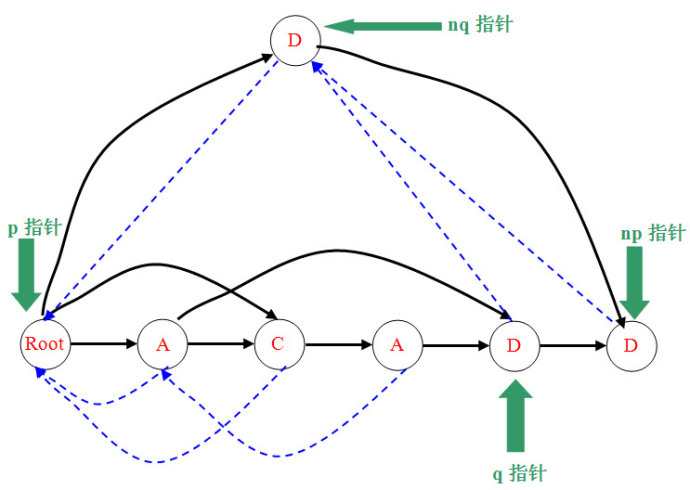
\includegraphics[scale=0.6]{suffix_auto.jpg}
  \caption{ACADD 构成的后缀自动机}
  \label{suffix_auto}
\end{figure}

我们发现 fail 构出一棵前缀树

和后缀树相同,为了使每个前缀都是叶子结点,我们不妨在串 s 前加入一个没出现的字符 '\#'

\begin{figure}
  \centering
  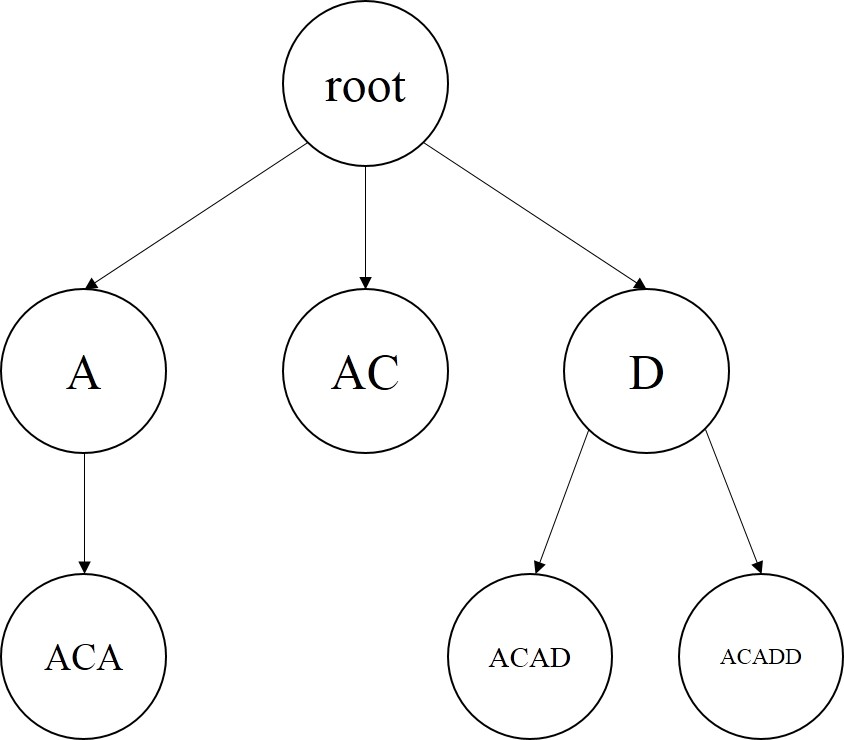
\includegraphics[scale=0.6]{suffix_auto2.jpg}
  \caption{串 ACADD 按 fail 构出的前缀树,与图 $\ref{suffix_auto}$ 对应}
  \label{suffix_auto2}
\end{figure}


\begin{figure}
  \centering
  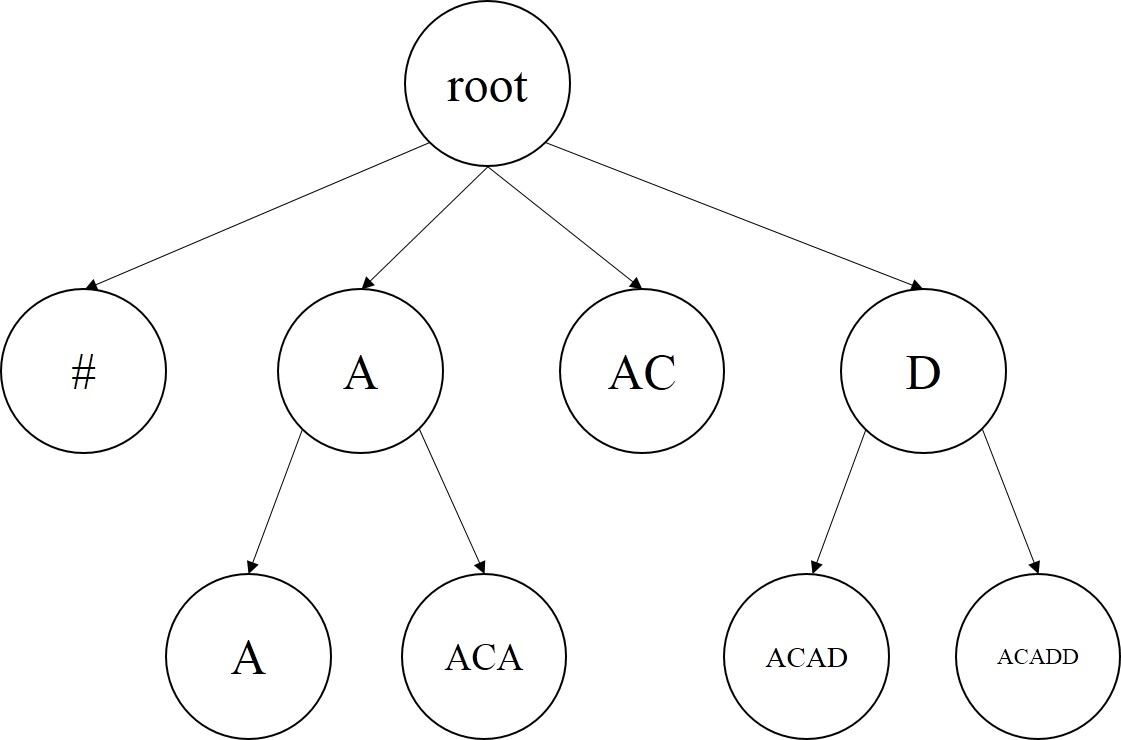
\includegraphics[scale=0.6]{suffix_auto3.jpg}
  \caption{串 \#ACADD 按 fail 构出的前缀树}
  \label{suffix_auto3}
\end{figure}

\subsection{回文树}

【URAL2040】Palindromes and Super Abilities 2

逐个添加字符串S里的字符 $S_1, S_2, ..., S_n$ 。每次添加字符后,他想知道添加字符后将出现多少个新的本质不同的回文子串。字符集为 $\{a, b\}$

\begin{lstlisting}[language=C++]
#include <bits/stdc++.h>
#define N 5000020

char st[N], answer[N];
int n;
 
struct PAM {
	int n, tot, last;
	int len[N], fail[N], next[N][2];
	void init() {
		n=0; tot=1;
		len[1]=-1; fail[1]=0;
		len[0]=+0; fail[0]=1;
		last=1;
	}
	int get_fail(int x) {
		for (; st[n-len[x]-1]!=st[n]; x=fail[x]);
		return x;
	}
	void insert(char c) {
		++n; int cur=get_fail(last); // 判断上一个串的前一个位置和新添加的位置是否相同,相同则说明构成回文。否则找 fail 指针。
		if (!next[cur][c]) {
			++tot;
			len[tot]=len[cur]+2;
			fail[tot]=next[get_fail(fail[cur])][c];
			next[cur][c]=tot;
			answer[n]='1';
		} else {
			answer[n]='0';
		}
		last=next[cur][c];
	}
} pam;
 
int main() {
	scanf("%s", st+1); n=strlen(st+1);
	pam.init();
	for (int i=1;i<=n;i++) pam.insert(st[i]-'a');
	puts(answer+1);
	return 0;
}
\end{lstlisting}

\section{数据结构}
\subsection{ST表}
\begin{lstlisting}[language=C++]
int Log[N],f[17][N];
int ask(int x,int y){
	int k=Log[y-x+1];
	return max(f[k][x],f[k][y-(1<<k)+1]);
}
int main(){
	for (int i=2;i<=n;i++)Log[i]=Log[i>>1]+1;
	for (int j=1;j<K;j++)
		for (int i=1;i+(1<<j-1)<=n;i++)
			f[j][i]=max(f[j-1][i],f[j-1][i+(1<<j-1)]);
}
\end{lstlisting}
\subsection{左偏树}

左偏树是一个可并堆。

下面的程序写的是一个小根堆,如果需要改成大根堆请在注释了 here 那行修改。

接口:

void push(const T \&x); 插入一个元素。

void merge(leftist \&x); 合并两个堆。注意,合并后原来那个堆将不可访问。

T top() const; 返回堆顶元素。

void pop(); 删除堆顶元素。

int size() const; 返回堆的大小。

\begin{lstlisting}[language=C++]
template <class T>
class leftist {
public:
    struct node {
        T key;
        int dist;
        node *l, *r;
    };
    leftist() : root(NULL), s(0) {}
    void push(const T &x) {
        leftist y;
        y.s = 1;
        y.root = new node;
        y.root -> key = x;
        y.root -> dist = 0;
        y.root -> l = y.root -> r = NULL;
        merge(y);
    }
    node* merge(node *x, node *y) {
        if (x == NULL) return y;
        if (y == NULL) return x;
        if (y -> key < x -> key) swap(x, y); //here
        x -> r = merge(x -> r, y);
        int ld = x -> l ? x -> l -> dist : -1;
        int rd = x -> r ? x -> r -> dist : -1;
        if (ld < rd) swap(x -> l, x -> r);
        if (x -> r == NULL) x -> dist = 0;
        else x -> dist = x -> r -> dist + 1;
        return x;
    }
    void merge(leftist &x) {
        root = merge(root, x.root);
        s += x.s;
    }
    T top() const {
        if (root == NULL) return T();
        return root -> key;
    }
    void pop() {
        if (root == NULL) return;
        node *p = root;
        root = merge(root -> l, root -> r);
        --s;
        delete p;
    }
    int size() const {
        return s;
    }
private:
    node* root;
    int s;
};
\end{lstlisting}
\subsection{线段树小技巧}
给定一个序列 $a$ ,寻找一个最大的 $i$ 使得 $i \leq y$ 且满足一些条件(如 $a[i] \geq w$ ,那么需要在线段树维护 $a$ 的区间最大值)
\begin{lstlisting}[language=C++]
int queryl(int p, int left, int right, int y, int w) {
	if (right <= y) {
		if (! __condition__ ) return -1;
		else if (left == right) return left;
	}
	int mid = (left + right) / 2;
	if (y <= mid) return queryl(p<<1|0, left, mid, y, w);
	int ret = queryl(p<<1|1, mid+1, right, y, w);
	if (ret != -1) return ret;
	return queryl(p<<1|0, left, mid, y, w);
}
\end{lstlisting}
给定一个序列 $a$ ,寻找一个最小的 $i$ 使得 $i \geq x$ 且满足一些条件(如 $a[i] \geq w$ ,那么需要在线段树维护 $a$ 的区间最大值)
\begin{lstlisting}[language=C++]
int queryr(int p, int left, int right, int x, int w) {
	if (left >= x) {
		if (! __condition__ ) return -1;
		else if (left == right) return left;
	}
	int mid = (left + right) / 2;
	if (x > mid) return queryr(p<<1|1, mid+1, right, x, w);
	int ret = queryr(p<<1|0, left, mid, x, w);
	if (ret != -1) return ret;
	return queryr(p<<1|1, mid+1, right, x, w);
}
\end{lstlisting}
\subsection{Splay}
接口: 

$\text{ADD x y d}$ : 将 $[x, y]$ 的所有数加上 $d$ 

$\text{REVERSE x y}$ : 将 $[x, y]$ 翻转 

$\text{INSERT x p}$ : 将 $p$ 插入到第 $x$ 个数的后面 

$\text{DEL x}$ : 将第 $x$ 个数删除
\begin{lstlisting}[language=C++]
struct SPLAY {
	struct NODE {
		int w, min;
		int son[2], size, father, rev, lazy;
	} node[N];
	int top, rt;
	void pushdown(int x) {
		if (!x) return;
		if (node[x].rev) {
			node[node[x].son[0]].rev ^= 1;
			node[node[x].son[1]].rev ^= 1;
			swap(node[x].son[0], node[x].son[1]);
			node[x].rev = 0;
		}
		if (node[x].lazy) {
			node[node[x].son[0]].lazy += node[x].lazy;
			node[node[x].son[1]].lazy += node[x].lazy;
			node[x].w += node[x].lazy;
			node[x].min += node[x].lazy;
			node[x].lazy = 0;
		}
	}
	void pushup(int x) {
		if (!x) return;
		pushdown(node[x].son[0]);
		pushdown(node[x].son[1]);
		node[x].size = node[node[x].son[0]].size + node[node[x].son[1]].size + 1;
		node[x].min = node[x].w;
		if (node[x].son[0]) node[x].min = min(node[x].min, node[node[x].son[0]].min);
		if (node[x].son[1]) node[x].min = min(node[x].min, node[node[x].son[1]].min);
	}
	void sc(int x, int y, int w) {
		node[x].son[w] = y;
		node[y].father = x;
		pushup(x);
	}
	void _ins(int w) {
		top++;
		node[top].w = node[top].min = w;
		node[top].son[0] = node[top].son[1] = 0;
		node[top].size = 1; node[top].father = 0; node[top].rev = 0;
	}
	void init() {
		top = 0;
		_ins(0); _ins(0); rt=1;
		sc(1, 2, 1);
	}
	void rotate(int x) {
		if (!x) return;
		int y = node[x].father;
		int w = node[y].son[1]==x;
		sc(y, node[x].son[w^1], w);
		sc(node[y].father, x, node[node[y].father].son[1]==y);
		sc(x, y, w^1);
	}
	int q[N];
	void flushdown(int x) {
		int t=0; for (; x; x=node[x].father) q[++t]=x;
		for (; t; t--) pushdown(q[t]);
	}
	void Splay(int x, int root=0) {
		flushdown(x);
		while (node[x].father != root) {
			int y=node[x].father;
			int w=node[y].son[1]==x;
			if (node[y].father != root && node[node[y].father].son[w]==y) rotate(y);
			rotate(x);
		}
	}
	int find(int k) {
		Splay(rt);
		while (1) {
			pushdown(rt);
			if (node[node[rt].son[0]].size+1==k) {
				Splay(rt);
				return rt;
			} else
			if (node[node[rt].son[0]].size+1<k) {
				k-=node[node[rt].son[0]].size+1;
				rt=node[rt].son[1];
			} else {
				rt=node[rt].son[0];
			}
		}
	}
	int split(int x, int y) {
		int fx = find(x);
		int fy = find(y+2);
		Splay(fx);
		Splay(fy, fx);
		return node[fy].son[0];
	}
	void add(int x, int y, int d) { //add d to each number in a[x]...a[y]
		int t = split(x, y);
		node[t].lazy += d;
		Splay(t); rt=t;
	}
	void reverse(int x, int y) { // reverse the x-th to y-th elements
		int t = split(x, y);
		node[t].rev ^= 1;
		Splay(t); rt=t;
	}
	void insert(int x, int p) { // insert p after the x-th element
		int fx = find(x+1);
		int fy = find(x+2);
		Splay(fx);
		Splay(fy, fx);
		_ins(p);
		sc(fy, top, 0);
		Splay(top); rt=top;
	}
	void del(int x) { // delete the x-th element in Splay
		int fx = find(x), fy = find(x+2);
		Splay(fx); Splay(fy, fx);
		node[fy].son[0] = 0;
		Splay(fy); rt=fy;
	}
} tree;
\end{lstlisting}

\subsection{可持久化Treap}
接口: 

void insert(int x, char c); 在当前第 $x$ 个字符后插入 $c$ 

void del(int x, int y); 删除第 $x$ 个字符到第 $y$ 个字符 

void copy(int l, int r, int x); 复制第 $l$ 个字符到第 $r$ 个字符,然后粘贴到第 $x$ 个字符后 

void reverse(int x, int y); 翻转第 $x$ 个到第 $y$ 个字符 

char query(int k); 表示询问当前第 $x$ 个字符是什么
\begin{lstlisting}[language=C++]
#define mod 1000000007
struct Treap {
	struct Node {
		char key;
		bool reverse;
		int lc, rc, size; // if size is long long, remember here
	} node[N];
	int n, root, rd;
	int Rand() { rd = (rd * 20372052LL + 25022087LL) % mod; return rd; }
	
	/*
	LL Rand() {
        LL t1 = rand() % 32768;
        LL t2 = rand() % 32768;
        LL t3 = rand() % 32768;
        LL t4 = rand() % 32768;
        return (((t1 * 32768) + t2) * 32768 + t3) * 32768 + t4;
    }
    */	
	
	void init() {
		n = root = 0;
	}
	inline int copy(int x) {
		node[++n] = node[x]; return n;
	}
	inline void pushdown(int x) {
		if (!node[x].reverse) return;
		if (node[x].lc) node[x].lc = copy(node[x].lc);
		if (node[x].rc) node[x].rc = copy(node[x].rc);
		swap(node[x].lc, node[x].rc);
		node[node[x].lc].reverse ^= 1;
		node[node[x].rc].reverse ^= 1;
		node[x].reverse = 0;
	}
	inline void pushup(int x) {
		node[x].size = node[node[x].lc].size + node[node[x].rc].size + 1;
	}
	int merge(int u, int v) {
		if (!u || !v) return u+v;
		pushdown(u); pushdown(v);
		int t = Rand() % (node[u].size + node[v].size), r;  // if size is long long, remember here
		if (t < node[u].size) {
			r = copy(u);
			node[r].rc = merge(node[u].rc, v);
		} else {
			r = copy(v);
			node[r].lc = merge(u, node[v].lc);
		}
		pushup(r);
		return r;
	}
	int split(int u, int x, int y) { // if size is long long, remember here
		if (x > y) return 0;
		pushdown(u);
		if (x == 1 && y == node[u].size) return u;
		if (y <= node[node[u].lc].size) return split(node[u].lc, x, y);
		int t = node[node[u].lc].size + 1; // if size is long long, remember here
		if (x > t) return split(node[u].rc, x-t, y-t);
		int num = copy(u);
		node[num].lc = split(node[u].lc, x, t-1);
		node[num].rc = split(node[u].rc, 1, y-t);
		pushup(num);
		return num;
	}
	void insert(int x, char c) {
		int t1 = split(root, 1, x), t2 = split(root, x+1, node[root].size);
		node[++n].key = c;
		node[n].lc = node[n].rc = 0;
		node[n].reverse = 0;
		pushup(n);
		root = merge(merge(t1, n), t2);
	}
	void del(int x, int y) {
		int t1 = split(root, 1, x-1), t2 = split(root, y+1, node[root].size);
		root = merge(t1, t2);
	}
	void copy(int l, int r, int x) {
		int t1 = split(root, 1, x), t2 = split(root, l, r), t3 = split(root, x+1, node[root].size);
		root = merge(merge(t1, t2), t3);
	}
	void reverse(int x, int y) {
		int t1 = split(root, 1, x-1), t2 = split(root, x, y), t3 = split(root, y+1, node[root].size);
		node[t2].reverse ^= 1;
		root = merge(merge(t1, t2), t3);
	}
	char query(int k) {
		int x = root;
		while (1) {
			pushdown(x);
			if (k <= node[node[x].lc].size) x = node[x].lc;
			else 
			if (k == node[node[x].lc].size + 1) return node[x].key;
			else
			k -= node[node[x].lc].size + 1, x = node[x].rc;
		}
	}
} treap;
\end{lstlisting}
\subsection{可持久化并查集}
接口:

void init() 初始化

void merge(int x, int y, int time) 在 time 时刻将 x 和 y 连一条边,注意加边顺序必须按 time 从小到大加边

void GetFather(int x, int time) 询问 time 时刻及以前的连边状态中,x所属的集合
\begin{lstlisting}[language=C++]
namespace pers_union {
	const int inf = 0x3f3f3f3f;
	int father[N], Father[N], Time[N];
	vector<int> e[N];
	void init() {
		for (int i=1;i<=n;i++) {
			father[i] = i;
			Father[i] = i;
			Time[i] = inf;
			e[i].clear();
			e[i].push_back(i);
		}
	}
	int getfather(int x) {
		return (father[x] == x) ? x : father[x] = getfather(father[x]);
	}
	int GetFather(int x, int time) {
		return (Time[x] <= time) ? GetFather(Father[x], time) : x;
	}
	void merge(int x, int y, int time) {
		int fx = getfather(x), fy = getfather(y);
		if (fx == fy) return;
		if (e[fx].size() > e[fy].size()) swap(fx, fy);
		father[fx] = fy;
		Father[fx] = fy;
		Time[fx] = time;
		for (int i=0;i<e[fx].size();i++) {
			e[fy].push_back(e[fx][i]);
		}
	}
};
\end{lstlisting}

\section{树}
\subsection{点分治}
初始化时须设置 $top = 1$ 。
\begin{lstlisting}[language=C++]
void addedge(int x, int y) {
	edge[++top].adj = y;
	edge[top].valid = 1;
	edge[top].next = gh[x];
	gh[x] = top;
}
void get_size(int x, int root=0) {
	size[x] = 1; son[x] = 0;
	int dd = 0;
	for (int p=gh[x]; p; p=edge[p].next)
		if (edge[p].adj != root && edge[p].valid) {
			get_size(edge[p].adj, x);
			size[x] += size[edge[p].adj];
			if (size[edge[p].adj] > dd) {
				dd = size[edge[p].adj];
				son[x] = edge[p].adj;
			}
		}
}
int getroot(int x) {
	get_size(x);
	int sz = size[x];
	while (size[son[x]] > sz/2)
		x = son[x];
	return x;
}
void dc(int x) {
	x = getroot(x);
	static int list[N], ltop;
	ltop = 0;
	for (int p=gh[x]; p; p=edge[p].next)
		if (edge[p].valid)
			list[++ltop] = p;
	clear();
	for (int i=1;i<=ltop;i++) {
		update();
		modify();
	}
	clear();
	for (int i=ltop;i>=1;i--) {
		update();
		modify();
	}
	//be careful about the root
	for (int p=gh[x]; p; p=edge[p].next)
		if (edge[p].valid) {
			edge[p].valid = 0;
			edge[p^1].valid = 0;
			dc(edge[p].adj);
		}
}
\end{lstlisting}
\subsection{Link Cut Tree}
接口: 

command(x, y) : 将 x 到 y 路径的 Splay Tree 分离出来。 

linkcut(u1, v1, u2, v2) : 将树中原有的边 (u1, v1) 删除,加入一条新边 (u2, v2) 
\begin{lstlisting}[language=C++]
struct DynamicTREE{
	struct NODE{
		int father, son[2], top, size, reverse;
	} splay[N];
	void init(int i, int fat) {
		splay[i].father = splay[i].son[0] = splay[i].son[1] = 0;
		splay[i].top = fat; splay[i].size = 1; splay[i].reverse = 0;
	}
	void pushdown(int x) {
		if (!x) return;
		int s0 = splay[x].son[0], s1 = splay[x].son[1];
		if (splay[x].reverse) {
			splay[s0].reverse ^= 1;
			splay[s1].reverse ^= 1;
			swap(splay[x].son[0], splay[x].son[1]);
			splay[x].reverse = 0;
		}
		s0 = splay[x].son[0], s1 = splay[x].son[1];
		splay[s0].top = splay[s1].top = splay[x].top;
	}
	void pushup(int x) {
		if (!x) return;
		pushdown(splay[x].son[0]);
		pushdown(splay[x].son[1]);
		splay[x].size = splay[splay[x].son[0]].size + splay[splay[x].son[1]].size + 1;
	}
	void sc(int x, int y, int w, bool Auto=true) {
		splay[x].son[w] = y;
		splay[y].father = x;
		if (Auto) {
			pushup(y);
			pushup(x);
		}
	}
	int top, tush[N];
	void flowdown(int x) {
		for (top=1; x; top++, x = splay[x].father) tush[top] = x;
		for (; top; top--) pushdown(tush[top]);
	}
	void rotate(int x) {
		if (!x) return;
		int y = splay[x].father;
		int w = splay[y].son[1] == x;
		pushdown(y);
		pushdown(x);
		sc(splay[y].father, x, splay[splay[y].father].son[1]==y, false);
		sc(y, splay[x].son[w^1], w, false);
		sc(x, y, w^1, false);
		pushup(y);
		pushup(x);
	}
	void Splay(int x, int rt=0) {
		if (!x) return;
		flowdown(x);
		while (splay[x].father != rt) {
			int y = splay[x].father;
			int w = splay[y].son[1]==x;
			if (splay[y].father != rt && splay[splay[y].father].son[w] == y) rotate(y);
			rotate(x);
		}
	}
	void split(int x) {
		int y = splay[x].son[1];
		if (!y) return;
		splay[y].father = 0;
		splay[x].son[1] = 0;
		splay[y].top = x;
		pushup(x);
	}
	void access(int x) {
		int y = 0;
		while (x) {
			Splay(x);
			split(x);
			sc(x, y, 1);
			Splay(x);
			y = x;
			x = splay[x].top;
		}
	}
	void changeroot(int x) {
		access(x);
		Splay(x);
		splay[x].reverse = 1;
		Splay(x);
	}
	void command(int x, int y, ...) {
		LL ans = 0;
		changeroot(x);
		access(y);
		Splay(x);
		//then you can modify the Splay Tree
	}
	void linkcut(int u1, int v1, int u2, int v2) {
		changeroot(u1);
		access(v1);
		Splay(u1); split(u1);
		splay[v1].top = 0;
		access(u2); changeroot(u2);
		access(v2); changeroot(v2);
		Splay(u2); Splay(v2);
		splay[v2].top = u2;
	}
} lct;
\end{lstlisting}

\subsection{求子树的直径}

树形 DP 。

答案保存在 $u, d$ 数组中。

$u[x].exc$ 表示切断 $x$ 与 $father[x]$ 的边, $father[x]$ 表示的那颗子树的直径。

$d[x].exc$ 表示切断 $x$ 与 $father[x]$ 的边, $x$ 表示的那颗子树的直径。

\begin{lstlisting}[language=C++]
#include <bits/stdc++.h>
 
#define N 200020
 
using namespace std;
 
vector<int> g[N];
int n, q, top;
int deep[N], father[N], son[N], size[N], Top[N], dfn[N], rdfn[N];
 
void dfs(int x, int root = 0) {
    deep[x] = deep[root] + 1;
    father[x] = root;
    son[x] = 0; size[x] = 1;
    if (root) g[x].erase(lower_bound(g[x].begin(), g[x].end(), root));
    // 去根
    int dd = 0;
    for (int i = 0; i < g[x].size(); ++i) {
        dfs(g[x][i], x);
        if (size[g[x][i]] > dd) {
            dd = size[g[x][i]];
            son[x] = g[x][i];
        }
        size[x] += size[g[x][i]];
    }
}
 
void split(int x, int tp) {
    dfn[x] = ++top; rdfn[top] = x; Top[x] = tp;
    if (son[x]) split(son[x], tp);
    for (int i = 0; i < g[x].size(); ++i)
        if (g[x][i] != son[x])
            split(g[x][i], g[x][i]);
}
 
struct data {
    int inc, inc_id;
    int exc, exc_l, exc_r;
    //inc 表示从该点出发可以走到的最远距离
    //inc_id 表示从该点出发可以走到的最远点的编号
    //exc 表示子树中两点最远距离
    //exc_l, exc_r 表示子树中两点取得最远距离的两点的编号
    data() {
        inc = inc_id = 0;
        exc = exc_l = exc_r = 0;
    }
} u[N], d[N];
 
int safe(int x, int y) {
    // 防止 inc_id = 0 的情况
    if (x) return x;
    return y;
}
 
void dfs1(int x) {
    d[x].inc = 1; d[x].inc_id = x;
    data mx1 = data(), mx2 = data();
    // mx1, mx2 表示儿子 inc 最大、第2大值,用于更新该点 exc
    for (int i = 0; i < g[x].size(); ++i) {
        dfs1(g[x][i]);
        if (d[g[x][i]].inc + 1 > d[x].inc) {
            d[x].inc = d[g[x][i]].inc + 1;
            d[x].inc_id = d[g[x][i]].inc_id;
        }
        if (d[g[x][i]].inc > mx1.inc) {
            mx2 = mx1;
            mx1 = d[g[x][i]];
        } else
        if (d[g[x][i]].inc > mx2.inc) {
            mx2 = d[g[x][i]];
        }
    }
    d[x].exc = mx1.inc + mx2.inc + 1;
    d[x].exc_l = safe(mx1.inc_id, x);
    d[x].exc_r = safe(mx2.inc_id, x);
    for (int i = 0; i < g[x].size(); ++i)
        if (d[g[x][i]].exc > d[x].exc) {
            d[x].exc = d[g[x][i]].exc;
            d[x].exc_l = d[g[x][i]].exc_l;
            d[x].exc_r = d[g[x][i]].exc_r;
        }
}
 
void dfs2(int x, data y) {
    u[x] = y;
    if (!y.exc) y.exc = 1, y.exc_l = y.exc_r = x;
    data mx1 = y, mx2 = data(), mx3 = data(), mxe1 = y, mxe2 = data();
    // mx1, mx2, mx3 表示根过来的子树中 inc 的最大、第2大、第3大值
    // mxe1, mxe2 表示根过来的子树中 exc 的最大、第2大值
    int mx1_id = -1, mx2_id = -1, mx3_id = -1, mxe1_id = -1, mxe2_id = -1;
    for (int i = 0; i < g[x].size(); ++i) {
        if (d[g[x][i]].inc > mx1.inc) {
            mx3 = mx2; mx3_id = mx2_id;
            mx2 = mx1; mx2_id = mx1_id;
            mx1 = d[g[x][i]]; mx1_id = i;
        } else
        if (d[g[x][i]].inc > mx2.inc) {
            mx3 = mx2; mx3_id = mx2_id;
            mx2 = d[g[x][i]]; mx2_id = i;
        } else
        if (d[g[x][i]].inc > mx3.inc) {
            mx3 = d[g[x][i]]; mx3_id = i;
        }
        if (d[g[x][i]].exc > mxe1.exc) {
            mxe2 = mxe1; mxe2_id = mxe1_id;
            mxe1 = d[g[x][i]]; mxe1_id = i;
        } else
        if (d[g[x][i]].exc > mxe2.exc) {
            mxe2 = d[g[x][i]]; mxe2_id = i;
        }
    }
    for (int i = 0; i < g[x].size(); ++i) {
        data z = data();
        if (i == mx1_id) {
            z.exc = mx2.inc + mx3.inc + 1;
            z.exc_l = safe(mx2.inc_id, x);
            z.exc_r = safe(mx3.inc_id, x);
        } else
        if (i == mx2_id) {
            z.exc = mx1.inc + mx3.inc + 1;
            z.exc_l = safe(mx1.inc_id, x);
            z.exc_r = safe(mx3.inc_id, x);
        } else {
            z.exc = mx1.inc + mx2.inc + 1;
            z.exc_l = safe(mx1.inc_id, x);
            z.exc_r = safe(mx2.inc_id, x);
        }
        if (i == mxe1_id) {
            if (mxe2.exc > z.exc) z = mxe2;
        } else {
            if (mxe1.exc > z.exc) z = mxe1;
        }
        if (i == mx1_id) {
            z.inc = mx2.inc + 1;
            z.inc_id = safe(mx2.inc_id, x);
        } else {
            z.inc = mx1.inc + 1;
            z.inc_id = safe(mx1.inc_id, x);
        }
        dfs2(g[x][i], z);
    }
}
\end{lstlisting}

\section{图}
\subsection{欧拉回路}
欧拉回路: 

无向图:每个顶点的度数都是偶数,则存在欧拉回路。 

有向图:每个顶点的入度 = 出度,则存在欧拉回路。 

欧拉路径: 

无向图:当且仅当该图所有顶点的度数为偶数,或者除了两个度数为奇数外其余的全是偶
数。 

有向图:当且仅当该图所有顶点出度 = 入度或者一个顶点出度 = 入度 + 1,另一个顶点入
度 = 出度 + 1,其他顶点出度 = 入度。

下面 $O(n + m)$ 求欧拉回路的代码中, $n$ 为点数, $m$ 为边数,若有解则依次输出经过的边的编号,若是无向图,则正数表示 $x$ 到 $y$ ,负数表示 $y$ 到 $x$ 。
\begin{lstlisting}[language=C++]
namespace UndirectedGraph{
	int n,m,i,x,y,d[N],g[N],v[M<<1],w[M<<1],vis[M<<1],nxt[M<<1],ed;
	int ans[M],cnt;
	void add(int x,int y,int z){
		d[x]++;
		v[++ed]=y;w[ed]=z;nxt[ed]=g[x];g[x]=ed;
	}
	void dfs(int x){
		for(int&i=g[x];i;){
			if(vis[i]){i=nxt[i];continue;}
			vis[i]=vis[i^1]=1;
			int j=w[i];
			dfs(v[i]);
			ans[++cnt]=j;
		}
	}
	void solve(){
		scanf("%d%d",&n,&m);
		for(i=ed=1;i<=m;i++)scanf("%d%d",&x,&y),add(x,y,i),add(y,x,-i);
		for(i=1;i<=n;i++)if(d[i]&1){puts("NO");return;}
		for(i=1;i<=n;i++)if(g[i]){dfs(i);break;}
		for(i=1;i<=n;i++)if(g[i]){puts("NO");return;}
		puts("YES");
		for(i=m;i;i--)printf("%d ",ans[i]);
	}
}
namespace DirectedGraph{
	int n,m,i,x,y,d[N],g[N],v[M],vis[M],nxt[M],ed;
	int ans[M],cnt;
	void add(int x,int y){
		d[x]++;d[y]--;
		v[++ed]=y;nxt[ed]=g[x];g[x]=ed;
	}
	void dfs(int x){
		for(int&i=g[x];i;){
			if(vis[i]){i=nxt[i];continue;}
			vis[i]=1;
			int j=i;
			dfs(v[i]);
			ans[++cnt]=j;
		}
	}
	void solve(){
		scanf("%d%d",&n,&m);
		for(i=1;i<=m;i++)scanf("%d%d",&x,&y),add(x,y);
		for(i=1;i<=n;i++)if(d[i]){puts("NO");return;}
		for(i=1;i<=n;i++)if(g[i]){dfs(i);break;}
		for(i=1;i<=n;i++)if(g[i]){puts("NO");return;}
		puts("YES");
		for(i=m;i;i--)printf("%d ",ans[i]);
	}
}
\end{lstlisting}
\subsection{最短路径}
\subsubsection{Dijkstra}
\begin{lstlisting}[language=C++]
#define LL long long

struct EDGE {
	int adj, w, next;
} edge[M*2];

typedef pair<LL, int> pli;
priority_queue <pli, vector<pli>, greater<pli> > q;

int n, top, gh[N];
LL dist[N];

void addedge(int x, int y, int w) {
	edge[++top].adj = y;
	edge[top].w = w;
	edge[top].next = gh[x];
	gh[x] = top;
}

LL dijkstra(int s, int t) {
	memset(dist, 63, sizeof(dist));
	memset(v, 0, sizeof(v));
	dist[s] = 0;
	q.push(make_pair(dist[s], s));
	while (!q.empty()) {
		LL dis = q.top().first;
		int x = q.top().second;
		q.pop();
		if (dis != dist[x]) continue;
		for (int p=gh[x]; p; p=edge[p].next) {
			if (dis + edge[p].w < dist[edge[p].adj]) {
				dist[edge[p].adj] = dis + edge[p].w;
				q.push(make_pair(dist[edge[p].adj], edge[p].adj));
			}
		}
	}
	return dist[t];
}
\end{lstlisting}
\subsubsection{SPFA}
\begin{lstlisting}[language=C++]
struct EDGE {
	int adj, w, next;
} edge[M*2];

int n,m,top,gh[N],v[N],cnt[N],q[N],dist[N],head,tail;

void addedge(int x, int y, int w) {
	edge[++top].adj = y;
	edge[top].w = w;
	edge[top].next = gh[x];
	gh[x] = top;
}

int spfa(int S, int T) {
	memset(v, 0, sizeof(v));
	memset(cnt, 0, sizeof(cnt));
	memset(dist, 63, sizeof(dist));
	head = 0, tail = 1;
	dist[S] = 0; q[1] = S;
	while (head != tail) {
		(head += 1) %= N;
		int x = q[head]; v[x] = 0;
		++cnt[x]; if (cnt[x] > n) return -1;
		for (int p=gh[x]; p; p=edge[p].next)
			if (dist[x] + edge[p].w < dist[edge[p].adj]) {
				dist[edge[p].adj] = dist[x] + edge[p].w;
				if (!v[edge[p].adj]) {
					v[edge[p].adj] = 1;
					(tail += 1) %= N;
					q[tail] = edge[p].adj;
				}
			}
	}
	return dist[T];
}
\end{lstlisting}
\subsection{K 短路}
接口:

kthsp::init(n) :初始化并设置节点个数为n

kthsp::add(x, y, w) :添加一条x到y的有向边

kthsp::work(S, T, k) :求S到T的第k短路
\begin{lstlisting}[language=C++]
#define N 200020
#define M 400020
#define LOGM 20
#define LL long long
#define inf (1LL<<61)

namespace pheap {
	struct Node {
		int next, son[2];
		LL val;
	} node[M*LOGM];
	int LOG[M];
	int root[M], size[M*LOGM], top;
	int add() {
		++top; assert(top < M*LOGM);
		node[top].next = node[top].son[0] = node[top].son[1] = 0;
		node[top].val = inf;
		return top;
	}
	int copy(int x) {
		int t = add();
		node[t] = node[x];
		return t;
	}
	void init() {
		memset(root, 0, sizeof(root));
		top = -1; add();
		LOG[1] = 0;
		for (int i=2;i<M;i++) LOG[i] = LOG[i>>1] + 1;
	}
	void upd(int x, int &next, LL &val) {
		if (val < node[x].val) {
			swap(val, node[x].val);
			swap(next, node[x].next);
		}
	}
	void insert(int x, int next, LL val) {
		int sz = size[root[x]] + 1;
		root[x] = copy(root[x]);
		size[root[x]] = sz; x = root[x];
		upd(x, next, val);
		for (int i=LOG[sz]-1;i>=0;i--) {
			int ind = (sz>>i)&1;
			node[x].son[ind] = copy(node[x].son[ind]);
			x = node[x].son[ind];
			upd(x, next, val);
		}
	}
};
 
namespace kthsp {
	using namespace pheap;
	struct EDGE {
		int adj, w, next;
	} edge[2][M];
	struct W {
		int x, y, w;
	} e[M];
	bool has_init = 0;
	int n, m, top[2], gh[2][N], v[N];
	LL dist[N];
	void init(int n1) {
		has_init = 1;
		n = n1; m = 0;
		memset(top, 0, sizeof(top));
		memset(gh, 0, sizeof(gh));
		for (int i=1;i<=n;i++) dist[i] = inf;
	}
	void addedge(int id, int x, int y, int w) {
		edge[id][++top[id]].adj = y;
		edge[id][top[id]].w = w;
		edge[id][top[id]].next = gh[id][x];
		gh[id][x] = top[id];
	}
	void add(int x, int y, int w) {
		assert(has_init);
		e[++m].x=x; e[m].y=y; e[m].w=w;
	}
	int best[N], bestw[N];
	typedef pair<LL, int> pli;
	priority_queue <pli, vector<pli>, greater<pli> > q;

	// you can replace dijkstra with SPFA or TOPSORT(DAG)
	void dijkstra(int S) {
		while (!q.empty()) q.pop();
		dist[S] = 0; q.push(make_pair(dist[S], S));
		while (!q.empty()) {
			LL dis = q.top().first;
			int x = q.top().second;
			q.pop();
			if (dist[x] != dis) continue;
			for (int p=gh[1][x]; p; p=edge[1][p].next) {
				int y = edge[1][p].adj;
				if (dist[x] + edge[1][p].w < dist[y]) {
					dist[y] = dist[x] + edge[1][p].w;
					best[y] = x;
					bestw[y] = p;
					q.push(make_pair(dist[y], y));
				}
			}
		}
	}
	void dfs(int x) {
		if (v[x]) return;
		v[x] = 1;
		if (best[x]) root[x] = root[best[x]];
		for (int p=gh[0][x]; p; p=edge[0][p].next)
			if (dist[edge[0][p].adj] != inf && bestw[x] != p) {
				insert(x, edge[0][p].adj, edge[0][p].w + dist[edge[0][p].adj] - dist[x]);
			}
		for (int p=gh[1][x]; p; p=edge[1][p].next)
			if (best[edge[1][p].adj] == x)
				dfs(edge[1][p].adj);
	}
	LL work(int S, int T, int k) {
		assert(has_init);
		n++; add(T, n, 0);
		if (S == T) k ++;
		T = n;
		for (int i=1;i<=m;i++) {
			addedge(0, e[i].x, e[i].y, e[i].w);
			addedge(1, e[i].y, e[i].x, e[i].w);
		}
		dijkstra(T);
		root[T] = 0; pheap::init();
		memset(v, 0, sizeof(v));
		dfs(T);
		while (!q.empty()) q.pop();
		if (k == 1) return dist[S];
		if (root[S]) q.push(make_pair(dist[S] + node[root[S]].val, root[S]));
		while (k--) {
			if (q.empty()) return inf;
			pli now = q.top(); q.pop();
			if (k == 1) return now.first;
			int x = node[now.second].next, u = node[now.second].son[0], v = node[now.second].son[1];
			if (root[x]) q.push(make_pair(now.first + node[root[x]].val, root[x]));
			if (u) q.push(make_pair(now.first - node[now.second].val + node[u].val, u));
			if (v) q.push(make_pair(now.first - node[now.second].val + node[v].val, v));
		}
		return 0;
	}
};
\end{lstlisting}
\subsection{Tarjan}
割点的判断:一个顶点 $u$ 是割点,当且仅当满足 $(1)$ 或 $(2)$ : \\
$(1)$ $u$ 为树根,且 $u$ 有多于一个子树(即:存在一个儿子 $v$ 使得 $dfn[u] + 1 \neq dfn[v]$ ) \\
$(2)$ $u$ 不为树根,且满足存在 $(u, v)$ 为树枝边( $u$ 为 $v$ 的父亲),使得 $dfn[u] \leq low[v]$ \\
桥的判断:一条无向边 $(u, v)$ 是桥,当且仅当 $(u, v)$ 为树枝边,满足 $dfn[u] < low[v]$ 
\begin{lstlisting}[language=C++]
struct EDGE { int adj, next; } edge[M];
int n, m, top, gh[N];
int dfn[N], low[N], cnt, ind, stop, instack[N], stack[N], belong[N];
void addedge(int x, int y) {
	edge[++top].adj = y;
	edge[top].next = gh[x];
	gh[x] = top;
}
void tarjan(int x) {
	dfn[x] = low[x] = ++ind;
	instack[x] = 1; stack[++stop] = x;
	for (int p=gh[x]; p; p=edge[p].next)
		if (!dfn[edge[p].adj]) {
			tarjan(edge[p].adj);
			low[x] = min(low[x], low[edge[p].adj]);
		} else if (instack[edge[p].adj]) {
			low[x] = min(low[x], dfn[edge[p].adj]);
		}
	if (dfn[x] == low[x]) {
		++cnt; int tmp=0;
		while (tmp!=x) {
			tmp = stack[stop--];
			belong[tmp] = cnt;
			instack[tmp] = 0;
		}
	}
}
\end{lstlisting}
\subsection{2-SAT}

\begin{lstlisting}[language=C++]
#define N number_of_vertex
#define M number_of_edges

struct MergePoint {
	struct EDGE {
		int adj, next;
	} edge[M];
	int ex[M], ey[M];
	bool instack[N];
	int gh[N], top, dfn[N], low[N], cnt, ind, stop, stack[N], belong[N];
	void init() {
		cnt = ind = stop = top = 0;
		memset(dfn, 0, sizeof(dfn));
		memset(instack, 0, sizeof(instack));
		memset(gh, 0, sizeof(gh));
	}
	void addedge(int x, int y) { //reverse
		std::swap(x, y);
		edge[++top].adj = y;
		edge[top].next = gh[x];
		gh[x] = top;
		ex[top] = x;
		ey[top] = y;
	}
	void tarjan(int x) {
		dfn[x] = low[x] = ++ind;
		instack[x] = 1; stack[++stop] = x;
		for (int p=gh[x]; p; p=edge[p].next)
			if (!dfn[edge[p].adj]) {
				tarjan(edge[p].adj);
				low[x] = std::min(low[x], low[edge[p].adj]);
			} else if (instack[edge[p].adj]) {
				low[x] = std::min(low[x], dfn[edge[p].adj]);
			}
		if (dfn[x] == low[x]) {
			++cnt; int tmp = 0;
			while (tmp!=x) {
				tmp = stack[stop--];
				belong[tmp] = cnt;
				instack[tmp] = 0;
			}
		}
	}
	void work() {
		for (int i = (__first__); i <= (__last__); ++i)
			if (!dfn[i])
				tarjan(i);
	}
} merge;
 
struct Topsort {
	struct EDGE {
		int adj, next;
	} edge[M];
	int n, top, gh[N], ops[N], deg[N], ans[N];
	std::queue<int> q;
	void init() {
		n = merge.cnt; top = 0;
		memset(gh, 0, sizeof(gh));
		memset(deg, 0, sizeof(deg));
	}
	void addedge(int x, int y) {
		if (x == y) return;
		edge[++top].adj = y;
		edge[top].next = gh[x];
		gh[x] = top;
		++deg[y];
	}
	void work() {
		for (int i = 1; i <= n; ++i)
			if (!deg[i])
				q.push(i);
		while (!q.empty()) {
			int x = q.front();
			q.pop();
			for (int p = gh[x]; p; p = edge[p].next)
				if (!--deg[edge[p].adj])
					q.push(edge[p].adj);
			if (ans[x]) continue;
			ans[x] = -1; //not selected
			ans[ops[x]] = 1; //selected
		}
	}
} ts;
\end{lstlisting}
调用示例:
\begin{lstlisting}[language=C++]
	merge.init();
	merge.addedge();
	merge.work();
	for (int i = 1; i <= n; ++i) {
		if (merge.belong[U(i, 0)] == merge.belong[U(i, 1)]) {
			puts("NO");
			return 0;
		}
		ts.ops[merge.belong[U(i, 0)]] = merge.belong[U(i, 1)];
		ts.ops[merge.belong[U(i, 1)]] = merge.belong[U(i, 0)];
	}
	ts.init();
	ts.work();
	puts("YES");
	for (int i = 1; i <= n; ++i) {
		int x = U(i, 0), y = U(i, 1);
		x = merge.belong[x], y = merge.belong[y];
		x = ts.ans[x], y = ts.ans[y];
		if (x == 1) puts("0 is selected");
		if (y == 1) puts("1 is selected");
	}
\end{lstlisting}

\subsection{统治者树(Dominator Tree)}
Dominator Tree 可以解决判断一类有向图必经点的问题。

idom[x] 表示离 x 最近的必经点(重编号后)。将 idom[x] 作为 x 的父亲,构成一棵 Dominator Tree

接口:

void dominator::init(int n); 初始化,有向图节点数为 $n$ 

void dominator::addedge(int u, int v); 添加一条有向边 (u, v)

void dominator::work(int root); 以 root 为根,建立一棵 Dominator Tree 

结果的返回:

在执行 dominator::work(int root); 后,树边保存在 vector <int> tree[N] 中
\begin{lstlisting}[language=C++]
namespace dominator {
	vector <int> g[N], rg[N], bucket[N], tree[N];
	int n, ind, idom[N], sdom[N], dfn[N], dsu[N], father[N], label[N], rev[N];
	void dfs(int x) {
		++ind;
		dfn[x] = ind; rev[ind] = x;
		label[ind] = dsu[ind] = sdom[ind] = ind;
		for (auto p : g[x]) {
			if (!dfn[p]) dfs(p), father[dfn[p]] = dfn[x];
			rg[dfn[p]].push_back(dfn[x]);
		}
	}
	void init(int n1) {
		n = n1; ind = 0;
		for (int i = 1; i <= n; ++i) {
			g[i].clear();
			rg[i].clear();
			bucket[i].clear();
			tree[i].clear();
			dfn[i] = 0;
		}
	}
	void addedge(int u, int v) {
		g[u].push_back(v);
	}
	int find(int x, int step=0) {
		if (dsu[x] == x) return step ? -1 : x;
		int y = find(dsu[x], 1);
		if (y < 0) return x;
		if (sdom[label[dsu[x]]] < sdom[label[x]])
			label[x] = label[dsu[x]];
		dsu[x] = y;
		return step ? dsu[x] : label[x];
	}
	void work(int root) {
		dfs(root); n = ind;
		for (int i = n; i; --i) {
			for (auto p : rg[i])
				sdom[i] = min(sdom[i], sdom[find(p)]);
			if (i > 1) bucket[sdom[i]].push_back(i);
			for (auto p : bucket[i]) {
				int u = find(p);
				if (sdom[p] == sdom[u]) idom[p] = sdom[p];
				else idom[p] = u;
			}
			if (i > 1) dsu[i] = father[i];
		}
		for (int i = 2; i <= n; ++i) {
			if (idom[i] != sdom[i])
				idom[i] = idom[idom[i]];
			tree[rev[i]].push_back(rev[idom[i]]);
			tree[rev[idom[i]]].push_back(rev[i]);
		}
	}
};
\end{lstlisting}
\subsection{网络流}
\subsubsection{最大流}
注意: \emph{top 要初始化为 1}
\begin{lstlisting}[language=C++]
struct EDGE { int adj, w, next; } edge[M];
int n, top, gh[N], nrl[N];
void addedge(int x, int y, int w) {
	edge[++top].adj = y;
	edge[top].w = w;
	edge[top].next = gh[x];
	gh[x] = top;
	edge[++top].adj = x;
	edge[top].w = 0;
	edge[top].next = gh[y];
	gh[y] = top;
}
int dist[N], q[N];
int bfs() {
	memset(dist, 0, sizeof(dist));
	q[1] = S; int head = 0, tail = 1; dist[S] = 1;
	while (head != tail) {
		int x = q[++head];
		for (int p=gh[x]; p; p=edge[p].next)
			if (edge[p].w && !dist[edge[p].adj]) {
				dist[edge[p].adj] = dist[x] + 1;
				q[++tail] = edge[p].adj;
			}
	}
	return dist[T];
}
int dinic(int x, int delta) {
	if (x==T) return delta;
	for (int& p=nrl[x]; p && delta; p=edge[p].next)
		if (edge[p].w && dist[x]+1 == dist[edge[p].adj]) {
			int dd = dinic(edge[p].adj, min(delta, edge[p].w));
			if (!dd) continue;
			edge[p].w -= dd;
			edge[p^1].w += dd;
			return dd;
		}
	return 0;
}
int work() {
	int ans = 0;
	while (bfs()) {
		memcpy(nrl, gh, sizeof(gh));
		int t; while (t = dinic(S, inf)) ans += t;
	}
	return ans;
}
\end{lstlisting}
\subsubsection{上下界有源汇网络流}
$T$ 向 $S$ 连容量为正无穷的边,将有源汇转化为无源汇。 

每条边容量减去下界,设 $in[i]$ 表示流入 $i$ 的下界之和减去流出 $i$ 的下界之和。  

新建超级源汇 $SS, TT$ ,对于 $in[i] > 0$ 的点, $SS$ 向 $i$ 连容量为 $in[i]$ 的边。对于 $in[i] < 0$ 的点, $i$ 向 $TT$ 连容量为 $-in[i]$ 的边。 

求出以 $SS, TT$ 为源汇的最大流,如果等于 $\Sigma in[i] (in[i]>0)$ ,则存在可行流。再求出 $S, T$ 为源汇的最大流即为最大流。 

费用流:建完图后等价于求以 $SS, TT$ 为源汇的费用流。
\subsubsection{上下界无源汇网络流}
1. 怎样求无源汇有上下界网络的可行流? 

由于有源汇的网络我们先要转化成无源汇,所以本来就无源汇的网络不用再作特殊处理。 

2. 怎样求无源汇有上下界网络的最大流、最小流? 

一种简易的方法是采用二分的思想,不断通过可行流的存在与否对 $(t, s)$ 边的上下界 $U, L$ 进行调整。求最大流时令 $U = \infty$ 并二分 $L$ ;求最小流时令 $L = 0$ 并二分 $U$ 。道理很简单,因为可行流的取值范围是一段连续的区间,我们只要通过二分找到有解和无解的分界线即可。

\begin{figure}[htbp]
  \centering
  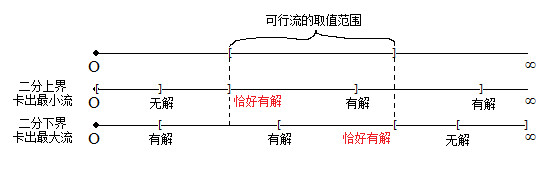
\includegraphics[scale=0.7]{nwf-1.jpg}
\end{figure}
\subsubsection{费用流}
注意: \emph{top 要初始化为 1}
\begin{lstlisting}[language=C++]
#define inf 0x3f3f3f3f
struct NetWorkFlow {
	struct EDGE {
		int adj, w, cost, next;
	} edge[M*2];
	int gh[N], q[N], dist[N], v[N], pre[N], prev[N], top;
	int S, T;
	void addedge(int x, int y, int w, int cost) {
		edge[++top].adj = y;
		edge[top].w = w;
		edge[top].cost = cost;
		edge[top].next = gh[x];
		gh[x] = top;
		edge[++top].adj = x;
		edge[top].w = 0;
		edge[top].cost = -cost;
		edge[top].next = gh[y];
		gh[y] = top;
	}
	void clear() {
		top = 1;
		memset(gh, 0, sizeof(gh));
	}
	int spfa() {
		memset(dist, 63, sizeof(dist));
		memset(v, 0, sizeof(v));
		int head = 0, tail = 1;
		q[1] = S; v[S] = 1; dist[S] = 0;
		while (head != tail) {
			(head += 1) %= N;
			int x = q[head];
			v[x] = 0;
			for (int p=gh[x]; p; p=edge[p].next)
				if (edge[p].w && dist[x] + edge[p].cost < dist[edge[p].adj]) {
					dist[edge[p].adj] = dist[x] + edge[p].cost;
					pre[edge[p].adj] = x;
					prev[edge[p].adj] = p;
					if (!v[edge[p].adj]) {
						v[edge[p].adj] = 1;
						(tail += 1) %= N;
						q[tail] = edge[p].adj;
					}
				}
		}
		return dist[T] != inf;
	}
	int work() {
		int ans = 0;
		while (spfa()) {
			int mx = inf;
			for (int x=T;x!=S;x=pre[x])
				mx = min(edge[prev[x]].w, mx);
			ans += dist[T] * mx; 
			for (int x=T;x!=S;x=pre[x]) {
				edge[prev[x]].w -= mx;
				edge[prev[x]^1].w += mx;
			}
		}
		return ans;
	}
} nwf;
\end{lstlisting}
\subsubsection{zkw费用流}
注意: \emph{top 要初始化为 1,不得用于有负权的图}
\begin{lstlisting}[language=C++]
#define inf 0x3f3f3f3f //modify if you use long long or double
template <class _tp>
struct NetWorkFlow {
	struct EDGE {
		int adj, next;
        _tp w, cost;
	} edge[M*2];
	int gh[N], top;
	int S, T;
	void addedge(int x, int y, _tp w, _tp cost) {
		edge[++top].adj = y;
		edge[top].w = w;
		edge[top].cost = cost;
		edge[top].next = gh[x];
		gh[x] = top;
		edge[++top].adj = x;
		edge[top].w = 0;
		edge[top].cost = -cost;
		edge[top].next = gh[y];
		gh[y] = top;
	}
	void clear() {
		top = 1;
		memset(gh, 0, sizeof(gh));
	}
	int v[N];
    _tp cost, d[N], slk[N];
	_tp aug(int x, _tp f) {
	    _tp left = f;
		if (x == T) {
			cost += f * d[S];
			return f;
		}
		v[x] = true;
		for (int p=gh[x]; p; p=edge[p].next)
			if (edge[p].w && !v[edge[p].adj]) {
				_tp t = d[edge[p].adj] + edge[p].cost - d[x];
				if (t == 0) {
					_tp delt = aug(edge[p].adj, min(left, edge[p].w));
					if (delt > 0) {
						edge[p].w -= delt;
						edge[p^1].w += delt;
						left -= delt;
					}
					if (left == 0) return f;
				} else {
				if (t < slk[edge[p].adj])
					slk[edge[p].adj] = t;
				}
			}
		return f-left;
	}
	bool modlabel() {
		_tp delt = inf;
		for (int i=1;i<=T;i++)
			if (!v[i]) {
				if (slk[i] < delt) delt = slk[i];
				slk[i] = inf;
			}
		if (delt == inf) return true;
		for (int i=1;i<=T;i++)
			if (v[i]) d[i] += delt;
		return false;
	}
	_tp work() {
		cost = 0;
		memset(d, 0, sizeof(d));
		memset(slk, 63, sizeof(slk));
		do {
			do {
				memset(v, 0, sizeof(v));
			} while (aug(S, inf));
		} while (!modlabel());
		return cost;
	}
};
NetWorkFlow<int> nwf;
\end{lstlisting}

\section{数学}
\subsection{扩展欧几里得解同余方程}
ans[] 保存的是循环节内所有的解
\begin{lstlisting}[language=C++]
int exgcd(int a,int b,int&x,int&y){
	if(!b)return x=1,y=0,a;
	int d=exgcd(b,a%b,x,y),t=x;
	return x=y,y=t-a/b*y,d;
}
void cal(ll a,ll b,ll n){//ax=b(mod n)
	ll x,y,d=exgcd(a,n,x,y);
	if(b%d)return;
	x=(x%n+n)%n;
	ans[cnt=1]=x*(b/d)%(n/d);
	for(ll i=1;i<d;i++)ans[++cnt]=(ans[1]+i*n/d)%n;
}
\end{lstlisting}
\subsection{同余方程组}
\begin{lstlisting} [language=C++]
int n,flag,k,m,a,r,d,x,y;
int main(){
	scanf("%d",&n);
	flag=k=1,m=0;
	while(n--){
		scanf("%d%d",&a,&r);//ans%a=r
		if(flag){
			d=exgcd(k,a,x,y);
			if((r-m)%d){flag=0;continue;}
			x=(x*(r-m)/d+a/d)%(a/d),y=k/d*a,m=((x*k+m)%y)%y;
			if(m<0)m+=y;
			k=y;
		}
	}
	printf("%d",flag?m:-1);//若flag=1,说明有解,解为ki+m,i为任意整数
}
\end{lstlisting}
\subsection{卡特兰数}
$h_1 = 1, h_n = \frac{h_{n-1}(4n-2)}{n+1} = \frac{C(2n, n)}{n+1} = C(2n, n) - C(2n, n-1)$ 

在一个格点阵列中,从 $(0, 0)$ 点走到 $(n, m)$ 点且不经过对角线 $x = y$ 的方案数 $(x > y)$ : 

$C(n+m-1, m) - C(n+m-1, m-1)$ 

在一个格点阵列中,从 $(0, 0)$ 点走到 $(n, m)$ 点且不穿过对角线 $x = y$ 的方案数 $(x \geq y)$ : 

 $C(n+m, m) - C(n+m, m-1)$ 
\subsection{斯特林数}
\subsubsection{第一类斯特林数}
第一类 Stirling 数 $S(p, k)$ 的一个组合学解释是:将 $p$ 个物体排成 $k$ 个非空循环排列的方法数。 

$S(p, k)$ 的递推公式: $S(p, k) = (p-1) S(p-1, k) + S(p-1, k-1), 1 \leq k \leq p-1$ 

边界条件: $S(p, 0) = 0, p \geq 1 \text{    } S(p, p) = 1, p \geq 0$
\subsubsection{第二类斯特林数}
第二类 Stirling 数 $S(p, k)$ 的一个组合学解释是:将 $p$ 个物体划分成 $k$ 个非空的不可辨别(可以理解为盒子没有编号)集合的方法数。

$S(p, k)$ 的递推公式: $S(p, k) = k S(p-1, k) + S(p-1, k-1), 1 \leq k \leq p-1$ 

边界条件: $S(p, 0) = 0, p \geq 1 \text{    } S(p, p) = 1, p \geq 0$

也有卷积形式: 

$$S(n, m) = \frac{1}{m!} \sum\limits_{k=0}^{m}(-1)^kC(m,k)(m-k)^n = \sum\limits_{k=0}^{m} \frac{(-1)^k(m-k)^n}{k!(m-k)!} = \sum\limits_{k=0}^{m}\frac{(-1)^k}{k!} \times \frac{(m-k)^n}{(m-k)!}$$
\subsection{错排公式}
$$D_1 = 0, D_2 = 1, D_n = (n-1)(D_{n-2} + D_{n-1})$$
\subsection{Lucas定理}
接口:  

初始化: void lucas::init(); 

计算 $C(n, m) \% mod$ 的值: LL lucas::Lucas(LL n, LL m);
\begin{lstlisting}[language=C++]
#define mod 110119
#define LL long long
namespace lucas {
	LL fac[mod+1], facv[mod+1];
	LL power(LL base, LL times) {
		LL ans = 1;
		while (times) {
			if (times&1) (ans *= base) %= mod;
			(base *= base) %= mod;
			times >>= 1;
		}
		return ans;
	}
	void init() {
		fac[0] = 1; for (int i=1;i<mod;i++) fac[i] = (fac[i-1] * i) % mod;
		facv[mod-1] = power(fac[mod-1], mod-2);
		for (int i=mod-2;i>=0;--i) facv[i] = (facv[i+1] * (i+1)) % mod;
	}
	LL C(unsigned LL n, unsigned LL m) {
		if (n < m) return 0;
		return (fac[n] * facv[m] % mod * facv[n-m] % mod) % mod;
	}
	LL Lucas(unsigned LL n, unsigned LL m)
	{
		if (m == 0) return 1;
		return (C(n%mod, m%mod) * Lucas(n/mod, m/mod)) %mod;
	}
};
\end{lstlisting}
\subsection{高斯消元}
\subsubsection{行列式}
\begin{lstlisting}[language=C++]
int ans = 1;
for (int i=0;i<n;i++) {
	for (int j=i;j<n;j++)
		if (g[j][i]) {
			for (int k=i;k<n;k++)
				swap(g[i][k], g[j][k]);
			if (j != i) ans *= -1;
			break;
		}
	if (g[i][i] == 0) {
		ans = 0;
		break;
	}
	for (int j=i+1;j<n;j++) {
		while (g[j][i]) {
			int t = g[i][i] / g[j][i];
			for (int k=i;k<n;k++)
				g[i][k] = (g[i][k] + mod - ((LL)t * g[j][k] % mod)) % mod;
			for (int k=i;k<n;k++)
				swap(g[i][k], g[j][k]);
			ans *= -1;
		}
	}
}
for (int i=0;i<n;i++)
	ans = ((LL)ans * g[i][i]) % mod;
ans = (ans % mod + mod) % mod;
printf("%d\n", ans);
\end{lstlisting}
\subsubsection{Matrix-Tree定理}
对于一张图,建立矩阵 $C$ , $C[i][i] = $ i 的度数,若 $i, j$ 之间有边,那么 $C[i][j] = -1$ ,否则为 $0$ 。这张图的生成树个数等于矩阵 $C$ 的 $n-1$ 阶行列式的值。
\subsection{调和级数}
$\sum\limits_{i=1}^n \frac{1}{i}$ 在 $n$ 较大时约等于 $ln(n) + r$ , $r$ 为欧拉常数,约等于 $0.5772156649015328$ 。
\subsection{曼哈顿距离的变换}
$\vert x_1 - x_2 \vert + \vert y_1 - y_2 \vert = max(\vert(x_1 + y_1) - (x_2 + y_2) \vert, \vert(x_1 - y_1) - (x_2 - y_2) \vert)$
\subsection{数论函数变换}

常见积性函数:

欧拉函数 $\phi(n)$ 为不超过 $n$ 的与 $n$ 互质的正整数个数

莫比乌斯函数 $\mu (n) = \left\{
	\begin{array}{lr}
	1, & \text{若} n = 1 \\
	(-1)^k, & \text{若} n \text{无平方数因数,且} n = p_1p_2 \cdots p_k \\
	0, & \text{若} n \text{有大于 1 的平方数因数} \\
	\end{array}
\right.
$

常见积性函数的性质:

$$n = \sum\limits_{d|n} \phi(d)$$

$$\sum\limits_{d|n} \mu(d) = \left\{
	\begin{array}{lr}
	1, & n = 1 \\
	0, & n > 1 \\
	\end{array}
\right.
$$

$$\sum\limits_{i=1}^{n} \sum\limits_{j=1}^{m} i \times j [gcd(i, j) = d] = \sum\limits_{i=1}^{\lfloor \frac{n}{d} \rfloor} \sum\limits_{j=1}^{\lfloor \frac{m}{d} \rfloor} id \times jd [gcd(i, j) = 1]$$

$$\phi(n) = \sum\limits_{d|n} \mu(d) \frac{n}{d}$$

\subsection{莫比乌斯反演}

$F(n)$ 和 $f(n)$ 是定义在非负整数集合上的两个函数,则:

$$F(n) = \sum\limits_{d|n}f(d) \Rightarrow f(n) = \sum\limits_{d|n} \mu(d) F(\frac{n}{d}) $$

$$F(n) = \sum\limits_{n|d}f(d) \Rightarrow f(n) = \sum\limits_{n|d} \mu(\frac{d}{n}) F(d) $$


\subsection{线性筛素数}
\begin{lstlisting}[language=C++]
mu[1]=phi[1]=1;top=0;
for (int i=2;i<N;i++) {
	if (!v[i]) prime[++top]=i, mu[i] = -1, phi[i] = i-1;
	for (int j=1;i*prime[j]<N && j<=top;j++) {
		v[i*prime[j]] = 1;
		if (i%prime[j]) {
			mu[i*prime[j]] = -mu[i];
			phi[i*prime[j]] = phi[i] * (prime[j]-1);
		} else {
			mu[i*prime[j]] = 0;
			phi[i*prime[j]] = phi[i] * prime[j];
			break;
		}
	}
}
\end{lstlisting}
\subsection{杜教筛}
getphi(t, x) 表示求 $\sum\limits_{i = 1}^{x} i^t \phi(i)$ 。

推导过程:

记 $S(n) = \sum\limits_{i = 1}^{n} f(i)$ ,取任意函数 $g$ 有恒等式
$$S(n) = \sum\limits_{i = 1}^{n} (f \cdot g) (i) - \sum\limits_{i = 2}^{n} g(i) S(\lfloor \frac{n}{i} \rfloor)$$

其中, $(f \cdot g)$ 表示 $f$ 和 $g$ 的狄利克雷卷积:即: $(f \cdot g) (n) = \sum\limits_{d | n} f(d)g(\frac{n}{d})$

关于恒等式的证明:

将 $\sum\limits_{i = 2}^{n} g(i)S(\lfloor \frac{n}{i} \rfloor)$ 移到左边去,即只需证

$$\sum\limits_{i = 1}^{n} (f \cdot g) (i) = \sum\limits_{i = 1}^{n} g(i) S(\lfloor \frac{n}{i} \rfloor)$$

将狄利克雷卷积展开,得:

$$\sum\limits_{i = 1}^{n} \sum\limits_{d | i} g(d) f(\frac{i}{d}) = \sum\limits_{i = 1}^{n} g(i) S(\lfloor \frac{n}{i} \rfloor)$$

即:

$$\sum\limits_{d = 1}^{n} g(d) \sum\limits_{i = 1}^{\lfloor \frac{n}{d} \rfloor} f(i) = \sum\limits_{i = 1}^{n} g(i) S(\lfloor \frac{n}{i} \rfloor)$$

显然相等,恒等式证完。

取 $f(i) = i^p \phi(i), g(i) = i^p$ ,则有:

$$S(n) = \sum\limits_{i = 1}^{n} i^p \phi(i) = \sum\limits_{i = 1}^{n} i^{p+1} - \sum\limits_{i = 2}^{n}i^pS(\lfloor \frac{n}{i} \rfloor)$$

其中有用到等式 $\sum\limits_{d | n} \phi(d) = n$

另外,莫比乌斯函数 $\mu(n)$ 也可以使用杜教筛求前缀和,记 $S'(n) = \sum\limits_{i = 1}^{n} \mu (i)$ ,则 $S'(n) = 1 - \sum\limits_{i = 2}^{n} S'(\lfloor \frac{n}{i} \rfloor)$


\begin{lstlisting}
#include <bits/stdc++.h>
 
#define N 5000020
#define LL long long
#define mod 1000000007
#define div2 ((mod+1)/2)
#define div6 ((mod+1)/6)
 
using namespace std;
 
int n, prime[N], v[N];
LL phi[3][N];
 
map<int, int> mp[3];
 
int sum(int t, int x) { //calculate 1^t + 2^t + ... + x^t
	if (t == 0) return x;
	if (t == 1) return 1ll * x * (x + 1) % mod * div2 % mod;
	if (t == 2) return 1ll * x * (x + 1) % mod * (2ll * x % mod + 1) % mod * div6 % mod;
	if (t == 3) return 1ll * x * x % mod * (x + 1) % mod * (x + 1) % mod * div2 % mod * div2 % mod;
}
 
int getphi(int t, int x) {
	if (x < N) return phi[t][x];
	if (mp[t].find(x) != mp[t].end()) return mp[t][x];
	LL ans = 0; int r = 0;
	for (int l = 2; l <= x; l = r + 1) {
		r = x / (x / l);
		ans += 1ll * getphi(t, x / l) * (((LL)sum(t, r) - sum(t, l - 1) + mod) % mod) % mod;
		ans %= mod;
	}
	ans = (LL)sum(t + 1, x) - ans + mod;
	ans %= mod;
	mp[t][x] = ans;
	return (int)ans;
}
 
int main() {
	memset(v, 0, sizeof(v));
	int top = 0;
	phi[0][1] = 1, phi[1][1] = 1, phi[2][1] = 1;
	for (int i = 2; i < N; ++i) {
		if (!v[i]) prime[++top] = i, phi[0][i] = i - 1, phi[1][i] = 1ll * i * phi[0][i] % mod, phi[2][i] = 1ll * i * phi[1][i] % mod;
		for (int j = 1; j <= top && prime[j] * i < N; ++j) {
			v[i * prime[j]] = 1;
			if (i % prime[j] == 0) {
				phi[0][i * prime[j]] = phi[0][i] * prime[j];
				phi[1][i * prime[j]] = 1ll * phi[1][i] * prime[j] % mod * prime[j] % mod;
				phi[2][i * prime[j]] = 1ll * phi[2][i] * prime[j] % mod * prime[j] % mod * prime[j] % mod;
				break;
			} else {
				phi[0][i * prime[j]] = phi[0][i] * (prime[j] - 1);
				phi[1][i * prime[j]] = 1ll * phi[1][i] * (prime[j] - 1) % mod * prime[j] % mod;
				phi[2][i * prime[j]] = 1ll * phi[2][i] * (prime[j] - 1) % mod * prime[j] % mod * prime[j] % mod;
			}
		}
	}
	for (int i = 2; i < N; ++i) {
		phi[0][i] = (phi[0][i] + phi[0][i - 1]) % mod;
		phi[1][i] = (phi[1][i] + phi[1][i - 1]) % mod;
		phi[2][i] = (phi[2][i] + phi[2][i - 1]) % mod;
	}
}
\end{lstlisting}
\subsection{FFT}

\subsubsection{普通FFT}

\begin{lstlisting}[language=C++]
namespace FFT {
	const int maxn = 65537;
	const double pi = acos(-1.0);

	struct comp {
		double real , imag;
		comp() {}
		comp(double real , double imag): real(real) , imag(imag) {}
		friend inline comp operator+(const comp &a , const comp &b) {
			return comp(a.real + b.real , a.imag + b.imag);
		}
		friend inline comp operator-(const comp &a , const comp &b) {
			return comp(a.real - b.real , a.imag - b.imag);
		}
		friend inline comp operator*(const comp &a , const comp &b) {
			return comp(a.real * b.real - a.imag * b.imag , a.real * b.imag + a.imag * b.real);
		}
	};

	comp A[maxn] , B[maxn];
	int rev[maxn], m, len;

	inline void init(int n) {
		for (m = 1, len = 0; m < n + n; m <<= 1 , len ++);
		for (int i = 0; i < m; ++i) rev[i] = (rev[i >> 1] >> 1) | ((i & 1) << (len - 1));
        for (int i = 0; i < m; ++i) A[i] = B[i] = comp(0, 0);
	}

	inline void dft(comp *a , int v) {
		for (int i = 0; i < m; ++i) if (i < rev[i]) swap(a[i] , a[rev[i]]);
		for (int s = 2; s <= m; s <<= 1) {
			comp g(cos(2 * pi / s) , v * sin(2 * pi / s));
			for (int k = 0; k < m; k += s) {
				comp w(1 , 0);
                for (int j = 0; j < s / 2; ++j) {
					comp &u = a[k + j + s / 2], &v = a[k + j];
					comp t = w * u;
					u = v - t;
					v = v + t;
					w = w * g;
				}
			}
		}
		if (v == -1)
			for (int i = 0; i < m; ++i) a[i].real /= m , a[i].imag /= m;
	}
}
\end{lstlisting}

\subsubsection{模任意素数FFT}

\emph{注意}:调用 $mulmod$ 前先调用 $init$ 。调用 $mulmod$ 前请确保 $a, b$  数组足够大(比 $2n$ 大的 $2$ 的整数次幂)且经过\emph{初始化}。

\begin{lstlisting}[language=C++]
namespace FFT {
	const long double pi = acos(-1.0);

	struct comp {
		long double real, imag;
		comp() {}
		comp(long double real, long double imag) : real(real), imag(imag) {}
		friend inline comp operator + (const comp &a, const comp &b) {
			return comp(a.real + b.real, a.imag + b.imag);
		}
		friend inline comp operator - (const comp &a, const comp &b) {
			return comp(a.real - b.real, a.imag - b.imag);
		}
		friend inline comp operator * (const comp &a, const comp &b) {
			return comp(a.real * b.real - a.imag * b.imag, a.real * b.imag + a.imag * b.real);
		}
		inline comp conj() {
			return comp(real, -imag);
		}
	};

	comp A[maxn], B[maxn];
	int rev[maxn], m, len;

	inline void init(int n) {
		for (m = 1, len = 0; m < n + n; m <<= 1, ++len);
		for (int i = 0; i < m; ++i) rev[i] = (rev[i >> 1] >> 1) | ((i & 1) << (len - 1));
		for (int i = 0; i < m; ++i) A[i] = B[i] = comp(0, 0);
	}

	inline void dft(comp *a, int v) {
		for (int i = 0; i < m; ++i) if (i < rev[i]) swap(a[i], a[rev[i]]);
		for (int s = 2; s <= m; s <<= 1) {
			comp g(cos(2 * pi / s), v * sin(2 * pi / s));
			for (int k = 0; k < m; k += s) {
				comp w(1, 0);
				for (int j = 0; j < s / 2; ++j) {
					comp &u = a[k + j + s / 2], &v = a[k + j];
					comp t = w * u;
					u = v - t;
					v = v + t;
					w = w * g;
				}
			}
		}
		if (v == -1)
			for (int i = 0; i < m; ++i) a[i].real /= m, a[i].imag /= m;
	}

	inline void mulmod(int *a, int *b, int *c) { // c = a * b % mod, c不能为a或b
		int M = sqrt(mod);
		for (int i = 0; i < m; ++i) {
			A[i] = comp(a[i] / M, a[i] % M);
			B[i] = comp(b[i] / M, b[i] % M);
		}	
		dft(A, 1); dft(B, 1);
		static comp t[maxn];
		for (int i = 0; i < m; ++i) {
			int j = i ? m - i : 0;
			t[i] = ((A[i] + A[j].conj()) * (B[j].conj() - B[i]) + (A[j].conj() - A[i]) * (B[i] + B[j].conj())) * comp(0, 0.25);
		}
		dft(t, -1);
		for (int i = 0; i < m; ++i)
			c[i] = (LL)(t[i].real + 0.5) % mod * M % mod;
		for (int i = 0; i < m; ++i) {
			int j = i ? m - i : 0;
			t[i] = (A[j].conj() - A[i]) * (B[j].conj() - B[i]) * comp(-0.25, 0) + comp(0, 0.25) * (A[i] + A[j].conj()) * (B[i] + B[j].conj());
		}
		dft(t, -1);
		for (int i = 0; i < m; ++i)
			c[i] = (1ll * c[i] + (LL)(t[i].real + 0.5) + (LL)(t[i].imag + 0.5) % mod * M * M % mod) % mod;
	}
};
\end{lstlisting}

\subsection{FWT}
给定长度为 $2^n$ 的序列 $A[0 \cdots 2^n-1], B[0 \cdots 2^n-1]$ ,求这两序列的

$or$ 卷积: $C_k = \sum\limits_{i \ or \ j=k} A_iB_j$

$and$ 卷积: $C_k = \sum\limits_{i \ and \ j=k} A_iB_j$

$xor$ 卷积: $C_k = \sum\limits_{i \ xor \ j=k} A_iB_j$

\begin{lstlisting}[language=C++]
void FWT(int *a, int n) {
    for (int d = 1; d < n; d <<= 1)
        for (int m = d << 1, i = 0; i < n; i += m)
            for (int j = 0; j < d; ++j) {
                int x = a[i + j], y = a[i + j + d];
                //or: a[i + j + d] = x + y;
                //and: a[i + j] = x + y;
                //xor: a[i + j] = x + y, a[i + j + d] = x - y;
                // 如答案要求取模,此处记得取模
            }
}

void UFWT(int *a, int n) {
    for (int d = 1; d < n; d <<= 1)
        for (int m = d << 1, i = 0; i < n; i += m)
            for (int j = 0; j < d; ++j) {
                int x = a[i + j], y = a[i + j + d];
                //or: a[i + j + d] = y - x;
                //and: a[i + j] = x - y;
                //xor: a[i + j] = (x + y) / 2, a[i + j + d] = (x - y) / 2;
                // 如答案要求取模,此处记得取模
            }
}
\end{lstlisting}

\subsection{求原根}
接口: LL p\_root(LL p); 

输入: 一个素数 $p$  

输出: $p$ 的原根
\begin{lstlisting}[language=C++]
#include <bits/stdc++.h>
#define LL long long

using namespace std;

vector <LL> a;

LL pow_mod(LL base, LL times, LL mod) {
	LL ret = 1;
	while (times) {
		if (times&1) ret = ret * base % mod;
		base = base * base % mod;
		times>>=1;
	}
	return ret;
}

bool g_test(LL g, LL p) {
	for (LL i = 0; i < a.size(); ++i)
		if (pow_mod(g, (p-1)/a[i], p) == 1) return 0;
	return 1;
}

LL p_root(LL p) {
	LL tmp = p - 1;
	for (LL i = 2; i <= tmp / i; ++i)
		if (tmp % i == 0) {
			a.push_back(i);
			while (tmp % i == 0)
				tmp /= i;
		}
	if (tmp != 1) a.push_back(tmp);
	LL g = 1;
	while (1) {
		if (g_test(g, p)) return g;
		++g;
	}
}

int main() {
	LL p;
	cin >> p;
	cout << p_root(p) << endl;
}
\end{lstlisting}
\subsection{NTT}
998244353 原根为 3 , 1004535809 原根为 3 ,786433 原根为 10 , 880803841 原根为 26 。

NTT 公式: $$ y_n = \sum\limits_{i = 0}^{d-1} x_i(g^{\frac{P-1}{d}})^{in} \ \text{mod} \ P $$

\begin{lstlisting}[language=C++]
#define mod 998244353
#define g 3
LL wi[N], wiv[N];
LL power(LL base, LL times) {
	LL ans = 1;
	while (times) {
		if (times&1) (ans *= base) %= mod;
		(base *= base) %= mod;
		times >>= 1;
	}
	return ans;
}
void transform(LL *x, int len) {
	for (int i=1,j=len/2;i<len-1;i++) {
		if (i<j) swap(x[i], x[j]);
		int k = len/2;
		while (j>=k) {
			j-=k;
			k/=2;
		}
		if (j<k) j+=k;
	}
}
void NTT(LL *x, int len, int reverse) {
	transform(x, len);
	for (int h=2;h<=len;h<<=1) {
		for (int i=0;i<len;i+=h) {
			LL w = 1, wn;
			if (reverse==1) wn = wi[h]; else wn = wiv[h];
			for (int j=i;j<i+h/2;j++) {
				LL u = x[j];
				LL v = (w * x[j+h/2]) % mod;
				x[j	] = (u + v) % mod;
				x[j+h/2] = (u - v + mod) % mod;
				(w *= wn) %= mod;
			}
		}
	}
	if (reverse == -1) {
		LL t = power(len, mod-2);
		for (int i=0;i<len;i++)
			(x[i] *= t) %= mod;
	}
}
LL A[N], B[N];
int main() {
	for (int i=1;i<N;i*=2) {
		wi[i] = power(g, (mod-1)/i);
		wiv[i] = power(wi[i], mod-2);
	}
	memset(A, 0, sizeof(A));
	memset(B, 0, sizeof(B));
	NTT(A, len, 1); NTT(B, len, 1);
	for (int i=0;i<len;i++) (A[i] *= B[i]) %= mod;
	NTT(A, len, -1);
}
\end{lstlisting}

\subsection{幂和}

$$\sum\limits_{i=1}^{n}i^1 = \frac{n(n+1)}{2} = \frac{1}{2}n^2 + \frac{1}{2}n$$

$$\sum\limits_{i=1}^{n}i^2 = \frac{n(n+1)(2n+1)}{6} = \frac{1}{3}n^3 + \frac{1}{2}n^2 + \frac{1}{6}n$$

$$\sum\limits_{i=1}^{n}i^3 = \frac{n^2(n+1)^2}{4} = \frac{1}{4}n^4 + \frac{1}{2}n^3 + \frac{1}{4}n^2$$

$$\sum\limits_{i=1}^{n}i^4 = \frac{n(n+1)(2n+1)(3n^2+3n-1)}{30} = \frac{1}{5}n^5 + \frac{1}{2}n^4 + \frac{1}{3}n^3 - \frac{1}{30}n$$

$$\sum\limits_{i=1}^{n}i^5 = \frac{n^2(n+1)^2(2n^2+2n-1)}{12} = \frac{1}{6}n^6 + \frac{1}{2}n^5 + \frac{5}{12}n^4 - \frac{1}{12}n^2$$

$$\sum\limits_{i=1}^{n}i^6 = \frac{n(n+1)(2n+1)(3n^4+6n^3-3n+1)}{42} = \frac{1}{7}n^7 + \frac{1}{2}n^6 + \frac{1}{2}n^5 - \frac{1}{6}n^3 + \frac{1}{42}n$$


\subsection{蔡勒公式}

$$w = (\lfloor \frac{c}{4} \rfloor - 2c + y + \lfloor \frac{y}{4} \rfloor + \lfloor \frac{13(m+1)}{5} \rfloor + d - 1) \text{ mod } 7$$

$w$ : 0星期日,1星期一,2星期二,3星期三,4星期四,5星期五,6星期六

$c$ : 年份前两位数

$y$ : 年份后两位数

$m$ : 月( $3 \leq m \leq 14$ ,即在蔡勒公式中,1、2月要看作上一年的13、14月来计算 )

$d$ : 日

\subsection{皮克定理}

给定顶点坐标均是整点(或正方形格点)的简单多边形(凸多边形),皮克定理说明了其面积 $S$ 和内部格点数目 $n$ 、边上格点数目 $s$ 的关系: $S = n + \frac{s}{2} + 1$ 。

\subsection{组合数 lcm}
$(n+1) lcm(C(n, 0), C(n,1),...,C(n,k)) = lcm(n+1, n, n-1, ..., n-k+1)$
\subsection{区间 lcm 的维护}
对于一个数,将其分解质因数,若有因子 $p^k$ ,那么拆分出 $k$ 个数 $p, p^2, ..., p^k$ ,权值都为 $p$ ,那么查询区间 $[l, r]$ 内所有数的 lcm 的答案 = 所有在该区间中出现过的数的权值之积,可持久化线段树维护即可。

\section{几何}

\subsection{二维计算几何}

\subsubsection{计算几何误差修正}

\begin{lstlisting}[language=C++]
const double pi = acos(-1.0);
const double eps = 1e-8;

inline double sqr(double x) {
	return x * x;
}

inline int sgn(double x) {
	if (x < -eps) return -1;
	return x > eps;
}

inline int cmp(double x, double y) {
	return sgn(x - y);
}
\end{lstlisting}

\subsubsection{计算几何点类}

成员函数:


$
\begin{array}{lr}
	\text{read()} & \text{输入一个点} \\
	\text{norm()} & \text{计算向量的模长} \\
\end{array}
$

相关函数:

$
\begin{array}{lr}
	\text{double sqr(double x)} & \text{计算一个数的平方} \\
	\text{double det(const point \&a, const point \&b)} & \text{计算两个向量的叉积} \\
	\text{double dot(const point \&a, const point \&b)} & \text{计算两个向量的点积} \\
	\text{double dis(const point \&a, const point \&b)} & \text{计算两个点的距离} \\
	\text{point rotate\_point(const point \&p, double A)} &\overrightarrow{OP}  \text{绕原点逆时针旋转A弧度} \\
	
\end{array}
$


\begin{lstlisting}[language=C++]
struct point {
	double x, y;
	point() : x(0), y(0) {}
	point(double a, double b) : x(a), y(b) {}
	inline void read() {
		scanf("%lf%lf", &x, &y);
	}
	inline friend point operator + (const point &a, const point &b) {
		return point(a.x + b.x, a.y + b.y);
	}
	inline friend point operator - (const point &a, const point &b) {
		return point(a.x - b.x, a.y - b.y);
	}
	inline friend bool operator == (const point &a, const point &b) {
		return cmp(a.x, b.x) == 0 && cmp(a.y, b.y) == 0;
	}
	inline friend point operator * (const double &a, const point &b) {
		return point(a * b.x, a * b.y);
	}
	inline friend point operator / (const point &a, const double &b) {
		return point(a.x / b, a.y / b);
	}
	inline double norm() const {
		return sqrt(sqr(x) + sqr(y));
	}
};

inline double det(const point &a, const point &b) {
	return a.x * b.y - a.y * b.x;
}

inline double dot(const point &a, const point &b) {
	return a.x * b.x + a.y * b.y;
}

inline double dis(const point &a, const point &b) {
	return (a - b).norm();
}

inline point rotate_point(const point &p, double A) {
	double tx = p.x, ty = p.y;
	return point(tx * cos(A) - ty * sin(A), tx * sin(A) + ty * cos(A));
}
\end{lstlisting}

\subsubsection{计算几何线段类}

相关函数:

bool point\_on\_segment(const point \&p, const segment \&l) 判断点p是否在线段l上(含端点)

double point\_to\_segment\_dist(const point \&p, const segment \&l) 求点p到线段l的距离

point sym\_point(const point \&p, const segment \&l) 求点p关于线段l的对称点

point point\_proj\_line(const point \&p, const segment \&l) 求点p到线段l的垂足

bool parallel(const segment \&a, const segment \&b) 判断线段a和线段b是否平行

point intersect\_point(const segment \&a, const segment \&b) 求直线a与直线b的交点(如要求线段a与线段b的交点,应先判断是否有)

bool is\_segment\_intersect(const segment \&l1, const segment \&l2) 判断线段a与线段b是否相交(含端点)(如不含端点,将 $\leq$ 改为 $<$ )

bool is\_line\_intersect\_segment(const point \&p1, const point \&p2, const segment \&l) 判断直线 $p_1p_2$ 是否与线段 $l$ 相交

bool is\_half\_line\_intersect\_segment(const point \&p1, const point \&p2, const segment \&l) 判断射线 $p_1p_2$ 是否与线段 $l$ 相交(含端点 $p_1$ )(如不含端点 $p_1$ ,将 $\geq$ 改为 $>$ )

\begin{lstlisting}[language=C++]
struct segment {
	point a, b;
	segment() {}
	segment(point x, point y) : a(x), b(y) {}
	void read() {
		a.read(); b.read();
	}
};

// determine whether point p is on segment l
bool point_on_segment(const point &p, const segment &l) {
	if ((cmp(l.a.x, p.x) <= 0 || cmp(l.b.x, p.x) <= 0) &&
		(cmp(l.a.x, p.x) >= 0 || cmp(l.b.x, p.x) >= 0) &&
		(cmp(l.a.y, p.y) <= 0 || cmp(l.b.y, p.y) <= 0) &&
		(cmp(l.a.y, p.y) >= 0 || cmp(l.b.y, p.y) >= 0)) {
		return sgn(det(p - l.a, l.b - l.a)) == 0;
	}
	return 0;
}

// determine the distance from the point p to segment l
double point_to_segment_dist(const point &p, const segment &l) {
	if (dis(l.a, l.b) < eps) return dis(p, l.a);
	if (sgn(dot(l.b - l.a, p - l.a)) < 0) return dis(l.a, p);
	if (sgn(dot(l.a - l.b, p - l.b)) < 0) return dis(l.b, p);
	return fabs(det(l.b - l.a, p - l.a)) / dis(l.b, l.a);
}

// determine the symmetrical point of point p on segment l
point sym_point(const point &p, const segment &l) {
	double a = l.b.x - l.a.x;
	double b = l.b.y - l.a.y;
	double t = ((p.x - l.a.x) * a + (p.y - l.a.y) * b) / (a * a + b * b);
	return point(2 * l.a.x + 2 * a * t - p.x, 2 * l.a.y + 2 * b * t - p.y);
}

point point_proj_line(const point &p, const segment &l) {
	double r = dot((l.b - l.a), (p - l.a)) / dot(l.b - l.a, l.b - l.a);
	return l.a + r * (l.b - l.a);
}

bool parallel(const segment &a, const segment &b) {
	return sgn(det(a.a - a.b, b.a - b.b)) == 0;
}

point intersect_point(const segment &a, const segment &b) {
	double s1 = det(a.a - b.a, b.b - b.a);
	double s2 = det(a.b - b.a, b.b - b.a);
	return (s1 * a.b - s2 * a.a) / (s1 - s2);
}

// determine whether segment l1 intersects with segment l2
bool is_segment_intersect(const segment &l1, const segment &l2) {
	const point &s1 = l1.a, &e1 = l1.b;
	const point &s2 = l2.a, &e2 = l2.b;
	if ( cmp( min(s1.x, e1.x), max(s2.x, e2.x) ) <= 0 &&
		 cmp( min(s1.y, e1.y), max(s2.y, e2.y) ) <= 0 &&
		 cmp( min(s2.x, e2.x), max(s1.x, e1.x) ) <= 0 &&
		 cmp( min(s2.y, e2.y), max(s1.y, e1.y) ) <= 0 &&
		 sgn( det(s2 - s1, e2 - s1) ) * sgn( det(s2 - e1, e2 - e1) ) <= 0 &&
		 sgn( det(s1 - s2, e1 - s2) ) * sgn( det(s1 - e2, e1 - e2) ) <= 0)
		return 1;
	return 0;
}

// determine whether line p1p2 intersects with segment l
bool is_line_intersect_segment(const point &p1, const point &p2, const segment &l) {
	assert(!(p1 == p2));
	return sgn( det(p1 - l.a, p2 - l.a) ) * sgn( det(p1 - l.b, p2 - l.b) ) <= 0;
}

// determine whether half-line p1p2 intersects with segment l
bool is_half_line_intersect_segment(const point &p1, const point &p2, const segment &l) {
	return is_line_intersect_segment(p1, p2, l) && sgn( det(p1 - l.a, p2 - l.a) ) * sgn( det(p1 - l.a, l.b - l.a) ) >= 0;
}

\end{lstlisting}

\subsection{凸包}
\begin{lstlisting}[language=C++]
typedef complex<int> point;
#define X real()
#define Y imag()
int n;
long long cross(point a,point b) {
	return 1ll * a.X * b.Y - 1ll * a.Y * b.X;
}
bool cmp(point a,point b) {
	return make_pair(a.X, a.Y) < make_pair(b.X, b.Y);
}
int convexHull(point p[],int n,point ch[]) {
	sort(p, p + n, cmp);
	int m = 0;
	for(int i = 0; i < n; ++i) {
		while(m > 1 && cross(ch[m-1] - ch[m-2], p[i] - ch[m-2]) <= 0) m--;
		ch[m++] = p[i];
	}
	int k = m;
	for(int i = n - 2; i >= 0; --i) {
		while(m > k && cross(ch[m-1] - ch[m-2], p[i] - ch[m-2]) <= 0) m--;
		ch[m++] = p[i];
	}
	if(n > 1) m--;
	return m;
}
\end{lstlisting}
\section{黑科技和杂项}
\subsection{找规律}
有些题目,只给一个正整数 $n$ ,然后要求输出一个答案。这时,我们可以暴力得到小数据的解,用高斯消元得到递推式,然后用矩阵快速幂求解。

使用方法: 

首先在 gauss.in 中输入小数据的解( $n = 1$ 时, $n = 2$ 时, $\cdots$ ) ,以 $EOF$ 结束。 

依次运行 gauss.cpp , matrix.cpp ,得到 matrix.out 

将 matrix.out 中的文件粘贴在 main.cpp 中相应的位置中。注意模数一定要是质数。


\begin{lstlisting}[language=C++]
//gauss.cpp
#include <bits/stdc++.h>
#define N 102
#define mod 1000000007
//caution: you can use this program iff mod is a prime.

using namespace std;

int n, m, k, a[N], g[N][N];

int power(int base, int times) {
	int ret = 1;
	while (times) {
		if (times & 1) ret = 1ll * ret * base % mod;
		base = 1ll * base * base % mod;
		times >>= 1;
	}
	return ret;
}

int test() {
	for (int i=0;i<m;i++) {
		for (int j=i;j<=m;j++)
			if (g[j][i]) {
				for (int k=i;k<=m;k++)
					swap(g[i][k], g[j][k]);
				break;
			}
		if (g[i][i] == 0)
			return 0;
		for (int j=i+1;j<n;j++) {
			while (g[j][i]) {
				int t = 1ll * g[i][i] * power(g[j][i], mod - 2) % mod;
				for (int k=i;k<n;k++)
					g[i][k] = (g[i][k] + mod - (1ll * t * g[j][k] % mod)) % mod;
				for (int k=i;k<=m;k++)
					swap(g[i][k], g[j][k]);
			}
		}
		int t = power(g[i][i], mod - 2);
		for (int j = 0; j <= m; ++j)
			g[i][j] = 1ll * g[i][j] * t % mod;
	}
	for (int i = m; i < n; ++i)
		if (g[i][m]) return 0;
	for (int i = m - 1; i >= 0; --i) {
		int t = power(g[i][i], mod - 2);
		g[i][i] = 1;
		g[i][m] = 1ll * g[i][m] * t % mod;
		for (int j = 0; j < i; ++j)
			g[j][m] = (g[j][m] + mod - 1ll * g[i][m] * g[j][i] % mod) % mod;
	}
	printf("%d\n", m);
	for (int i = 0; i < m; ++i)
		printf("%d ", g[i][m]);
	puts("");
	for (int i = 0; i < m - 1; ++i)
		printf("%d ", a[i]);
	puts("1");
	return 1;
}

int main() {
	freopen("gauss.in", "r", stdin);
	freopen("gauss.out", "w", stdout);
	k = 0;
	while (~scanf("%d", &a[k++])) ;
	for (int sm = 1; sm <= k - sm; ++sm) {
		n = k - sm - 1;
		m = sm + 1;
		for (int i = 0; i < n; ++i) {
			for (int j = 0; j <= sm; ++j)
				g[i][j] = a[i + j];
			g[i][m] = 1;
			swap(g[i][m - 1], g[i][m]);
		}
		if (test()) return 0;
	}
	puts("no solution");
	return 0;
}
\end{lstlisting}

\begin{lstlisting}[language=C++]
//matrix.cpp
#include <bits/stdc++.h>
#define N 102
using namespace std;

int n, a[N];

int main() {
    freopen("gauss.out", "r", stdin);
    freopen("matrix.out", "w", stdout);
    scanf("%d", &n);
    for (int i = 0; i < n; ++i) scanf("%d", &a[i]);
    printf("#define M %d\n", n);
    printf("const int trans[M][M] = {\n");
    for (int i = 0; i < n; ++i) {
        printf("\t{");
        for (int j = 0; j < n; ++j) {
            int t;
            if (j < n - 2) t = i == j + 1;
            else if (j == n - 2) t = a[i];
            else t = i == n - 1;
            printf("%s%d", j == 0 ? "" : ", ", t);
        }
        printf("}%s\n", i == n - 1 ? "" : ",");
    }
    printf("};\n");
    printf("const int pref[M] = {");
    for (int i = 0; i < n; ++i) {
        int x;
        scanf("%d", &x);
        printf("%d%s", x, i == n - 1 ? "};\n" : ", ");
    }
    return 0;
}
\end{lstlisting}

\begin{lstlisting}[language=C++]
//main.cpp
#include <bits/stdc++.h>
using namespace std;

/* paste matrix.out here. */

#define mod 1000000007

struct Matrix {
    int c[M][M];
    void clear() { memset(c, 0, sizeof(c)); }
    void identity() { clear(); for (int i = 0; i < M; ++i) c[i][i] = 1; }
    void base() { memcpy(c, trans, sizeof(trans)); }
    friend Matrix operator * (const Matrix &a, const Matrix &b) {
        Matrix c; c.clear();
        for (int i = 0; i < M; ++i)
            for (int j = 0; j < M; ++j)
                for (int k = 0; k < M; ++k)
                    c.c[i][j] = (c.c[i][j] + 1ll * a.c[i][k] * b.c[k][j] % mod) % mod;
        return c;
    }
} start, base;

Matrix power(Matrix base, int times) {
    Matrix ret; ret.identity();
    while (times) {
        if (times & 1) ret = ret * base;
        base = base * base;
        times >>= 1;
    }
    return ret;
}

int main() {
    int tot;
    scanf("%d", &tot);
    while (tot--) {
        int n;
        scanf("%d", &n);
        start.clear();
        for (int i = 0; i < M; ++i) start.c[0][i] = pref[i];
        base.base();
        base = power(base, n - 1);
        start = start * base;
        printf("%d\n", start.c[0][0]);
    }
    return 0;
}
\end{lstlisting}

\subsection{分数类}

\begin{lstlisting}[language=C++]
#define LL long long

struct frac {
	LL x, y;
	frac(LL _x = 0, LL _y = 1) {
		x = _x;
		y = _y;
		LL g = __gcd(abs(x), abs(y));
		x /= g;
		y /= g;
		if (y < 0) {
			x = -x;
			y = -y;
		}
	}

	inline friend frac operator + (const frac &lhs, const frac &rhs) {
		return frac(lhs.x * rhs.y + rhs.x * lhs.y, lhs.y * rhs.y);
	}

	inline friend frac operator - (const frac &lhs, const frac &rhs) {
		return frac(lhs.x * rhs.y - rhs.x * lhs.y, lhs.y * rhs.y);
	}

	inline friend frac operator - (const frac &lhs) {
		return frac(-lhs.x, lhs.y);
	}

	inline friend frac operator * (const frac &lhs, const frac &rhs) {
		return frac(lhs.x * rhs.x, lhs.y * rhs.y);
	}

	inline friend frac operator / (const frac &lhs, const frac &rhs) {
		return frac(lhs.x * rhs.y, lhs.y * rhs.x);
	}

	inline friend bool operator == (const frac &lhs, const frac &rhs) {
		return lhs.x * rhs.y == rhs.x * lhs.y;
	}

	inline friend bool operator != (const frac &lhs, const frac &rhs) {
		return lhs.x * rhs.y != rhs.x * lhs.y;
	}

	inline friend bool operator < (const frac &lhs, const frac &rhs) {
		return lhs.x * rhs.y < rhs.x * lhs.y;
	}

	inline friend bool operator > (const frac &lhs, const frac &rhs) {
		return lhs.x * rhs.y > rhs.x * lhs.y;
	}

	inline friend bool operator <= (const frac &lhs, const frac &rhs) {
		return lhs.x * rhs.y <= rhs.x * lhs.y;
	}

	inline friend bool operator >= (const frac &lhs, const frac &rhs) {
		return lhs.x * rhs.y >= rhs.x * lhs.y;
	}

	inline void print() const {
		printf("%lld/%lld\n", x, y);
	}
};
\end{lstlisting}

\subsection{高精度计算}
\begin{lstlisting}[language=C++]
#include<algorithm>
using namespace std;
const int N_huge=850,base=100000000;
char s[N_huge*10];
struct huge{
	typedef long long value;
	value a[N_huge];int len;
	void clear(){len=1;a[len]=0;}
	huge(){clear();}
	huge(value x){*this=x;}
	huge operator =(huge b){
		len=b.len;for (int i=1;i<=len;++i)a[i]=b.a[i]; return *this;
	}
	huge operator =(value x){
		len=0;
		while (x)a[++len]=x%base,x/=base;
		if (!len)a[++len]=0;
		return *this;
	}
	huge operator +(huge b){
		int L=len>b.len?len:b.len;huge tmp;
		for (int i=1;i<=L+1;++i)tmp.a[i]=0;
		for (int i=1;i<=L;++i){
			if (i>len)tmp.a[i]+=b.a[i];
			else if (i>b.len)tmp.a[i]+=a[i];
			else {
				tmp.a[i]+=a[i]+b.a[i];
				if (tmp.a[i]>=base){
					tmp.a[i]-=base;++tmp.a[i+1];
				}
			}
		}
		if (tmp.a[L+1])tmp.len=L+1;
			else tmp.len=L;
		return tmp;
	}
	huge operator -(huge b){
		int L=len>b.len?len:b.len;huge tmp;
		for (int i=1;i<=L+1;++i)tmp.a[i]=0;
		for (int i=1;i<=L;++i){
			if (i>b.len)b.a[i]=0;
			tmp.a[i]+=a[i]-b.a[i];
			if (tmp.a[i]<0){
				tmp.a[i]+=base;--tmp.a[i+1];
			}
		}
		while (L>1&&!tmp.a[L])--L;
		tmp.len=L;
		return tmp;
	}
	huge operator *(huge b){
		int L=len+b.len;huge tmp;
		for (int i=1;i<=L;++i)tmp.a[i]=0;
		for (int i=1;i<=len;++i)
			for (int j=1;j<=b.len;++j){
				tmp.a[i+j-1]+=a[i]*b.a[j];
				if (tmp.a[i+j-1]>=base){
					tmp.a[i+j]+=tmp.a[i+j-1]/base;
					tmp.a[i+j-1]%=base;
				}
			}
		tmp.len=len+b.len;
		while (tmp.len>1&&!tmp.a[tmp.len])--tmp.len;
		return tmp;
	}
	pair<huge,huge> divide(huge a,huge b){
		int L=a.len;huge c,d;
		for (int i=L;i;--i){
		c.a[i]=0;d=d*base;d.a[1]=a.a[i];
			int l=0,r=base-1,mid;
			while (l<r){
				mid=(l+r+1)>>1;
				if (b*mid<=d)l=mid;
					else r=mid-1;
			}
			c.a[i]=l;d-=b*l;
		}
		while (L>1&&!c.a[L])--L;c.len=L;
		return make_pair(c,d);
	}
	huge operator /(value x){
		value d=0;huge tmp;
		for (int i=len;i;--i){
			d=d*base+a[i];
			tmp.a[i]=d/x;d%=x;
		}
		tmp.len=len;
		while (tmp.len>1&&!tmp.a[tmp.len])--tmp.len;
		return tmp;
	}
	value operator %(value x){
		value d=0;
		for (int i=len;i;--i)d=(d*base+a[i])%x;
		return d;
	}
	huge operator /(huge b){return divide(*this,b).first;}
	huge operator %(huge b){return divide(*this,b).second;}
	huge &operator +=(huge b){*this=*this+b;return *this;}
	huge &operator -=(huge b){*this=*this-b;return *this;}
	huge &operator *=(huge b){*this=*this*b;return *this;}
	huge &operator ++(){huge T;T=1;*this=*this+T;return *this;}
	huge &operator --(){huge T;T=1;*this=*this-T;return *this;}
	huge operator ++(int){huge T,tmp=*this;T=1;*this=*this+T;return tmp;}
	huge operator --(int){huge T,tmp=*this;T=1;*this=*this-T;return tmp;}
	huge operator +(value x){huge T;T=x;return *this+T;}
	huge operator -(value x){huge T;T=x;return *this-T;}
	huge operator *(value x){huge T;T=x;return *this*T;}
	huge operator *=(value x){*this=*this*x;return *this;}
	huge operator +=(value x){*this=*this+x;return *this;}
	huge operator -=(value x){*this=*this-x;return *this;}
	huge operator /=(value x){*this=*this/x;return *this;}
	huge operator %=(value x){*this=*this%x;return *this;}
	bool operator ==(value x){huge T;T=x;return *this==T;}
	bool operator !=(value x){huge T;T=x;return *this!=T;}
	bool operator <=(value x){huge T;T=x;return *this<=T;}
	bool operator >=(value x){huge T;T=x;return *this>=T;}
	bool operator <(value x){huge T;T=x;return *this<T;}
	bool operator >(value x){huge T;T=x;return *this>T;}
	bool operator <(huge b){
		if (len<b.len)return 1;
		if (len>b.len)return 0;
		for (int i=len;i;--i){
			if (a[i]<b.a[i])return 1;
			if (a[i]>b.a[i])return 0;
		}
		return 0;
	}
	bool operator ==(huge b){
		if (len!=b.len)return 0;
		for (int i=len;i;--i)
			if (a[i]!=b.a[i])return 0;
		return 1;
	}
	bool operator !=(huge b){return !(*this==b);}
	bool operator >(huge b){return !(*this<b||*this==b);}
	bool operator <=(huge b){return (*this<b)||(*this==b);}
	bool operator >=(huge b){return (*this>b)||(*this==b);}
	void str(char s[]){
		int l=strlen(s);value x=0,y=1;len=0;
		for (int i=l-1;i>=0;--i){
			x=x+(s[i]-'0')*y;y*=10;
			if (y==base)a[++len]=x,x=0,y=1;
		}
		if (!len||x)a[++len]=x;
	}
	void read(){
		scanf("%s",s);this->str(s);
	}
	void print(){
		printf("%d",(int)a[len]);
		for (int i=len-1;i;--i){
			for (int j=base/10;j>=10;j/=10){
				if (a[i]<j)printf("0");
					else break;
			}
			printf("%d",(int)a[i]);
		}
		printf("\n");
	}
}f[1005];
int main(){
	f[1]=f[2]=1;
	for(int i=3;i<=1000;i++)f[i]=f[i-1]+f[i-2];
}
\end{lstlisting}

\subsection{读入优化}

\subsubsection{普通读入优化}

\begin{lstlisting}[language=C++]
#define rd RD<int>
#define rdll RD<long long>
template <typename Type>
inline Type RD() {
    Type x = 0;
    int flag = 0;
    char c = getchar();
    while (!isdigit(c) && c != '-')
        c = getchar();
    (c == '-') ? (flag = 1) : (x = c - '0');
    while (isdigit(c = getchar()))
        x = x * 10 + c - '0';
    return flag ? -x : x;
}
inline char rdch() {
    char c = getchar();
    while (!isalpha(c)) c = getchar();
    return c;
}
\end{lstlisting}

\subsubsection{HDU 专用读入优化}

不支持负数。

\begin{lstlisting}[language=C++]
const int S = 2000000;

char s[S], *h = s+S, *t = h;

inline char getchr(void) {
	if(h == t) fread(s, 1, S, stdin), h = s;
	return *h++;
}

inline int rd(void) {
	char c = getchr();
	for (; !isdigit(c); c = getchr()) ;
	int x = 0;
	for (; isdigit(c); c = getchr()) x = x * 10 + c - '0';
	return x;
}
\end{lstlisting}

\subsection{位运算及其运用}

\subsubsection{枚举子集}

枚举 $i$ 的非空子集 $j$

\begin{lstlisting}[language=C++]
for (int j = i; j; j = (j - 1) & i);
\end{lstlisting}

\subsubsection{求 1 的个数}

\begin{lstlisting}[language=C++]
int __builtin_popcount(unsigned int x);
\end{lstlisting}

\subsubsection{求前缀 0 的个数}

\begin{lstlisting}[language=C++]
int __builtin_clz(unsigned int x);
\end{lstlisting}

\subsubsection{求后缀 0 的个数}

\begin{lstlisting}[language=C++]
int __builtin_ctz(unsigned int x);
\end{lstlisting}

\section{Sublime Text}

\subsection{License}

\begin{lstlisting}
-- BEGIN LICENSE --
Michael Barnes
Single User License
EA7E-821385
8A353C41 872A0D5C DF9B2950 AFF6F667
C458EA6D 8EA3C286 98D1D650 131A97AB
AA919AEC EF20E143 B361B1E7 4C8B7F04
B085E65E 2F5F5360 8489D422 FB8FC1AA
93F6323C FD7F7544 3F39C318 D95E6480
FCCC7561 8A4A1741 68FA4223 ADCEDE07
200C25BE DBBC4855 C4CFB774 C5EC138C
0FEC1CEF D9DCECEC D3A5DAD1 01316C36
-- END LICENSE --
\end{lstlisting}

\subsection{Preferences.sublime-settings}

\begin{lstlisting}
{
	"font_size": 13, 
	"show_encoding": true,
	"auto_match_enabled": false
}
\end{lstlisting}


\end{document}
















